\documentclass[10pt,DIV12,a4paper,openright,twoside,abstracton]{scrreprt}
\usepackage{fixltx2e}
\usepackage[T1]{fontenc}
\usepackage{textcomp}
\usepackage{isabelle}
\isatagannexa
  \usepackage{omg}
  \usepackage{draftwatermark}
  \SetWatermarkAngle{55}
  \SetWatermarkLightness{.9}
  \SetWatermarkFontSize{3cm}
  \SetWatermarkScale{1.4}
  \SetWatermarkText{\textbf{\textsf{Draft Proposal}}}
\endisatagannexa
\usepackage[nocolortable, noaclist,isasymonly,nocolor]{hol-ocl-isar}
\renewcommand{\lfloor}{\isasymHolOclLiftLeft}
\renewcommand{\rfloor}{\isasymHolOclLiftRight}
\renewcommand{\lceil}{\isasymHolOclDropLeft}
\renewcommand{\rceil}{\isasymHolOclDropRight}
\renewcommand{\oclkeywordstyle}{\bfseries}
\renewcommand{\javakeywordstyle}{\bfseries}
\renewcommand{\smlkeywordstyle}{\bfseries}
\renewcommand{\holoclthykeywordstyle}{}

\usepackage{lstisar}
\usepackage{railsetup}
\usepackage[]{mathtools}
\usepackage{booktabs}
\usepackage{graphicx}
\usepackage[numbers, sort&compress, sectionbib]{natbib}
\usepackage{chapterbib}
\usepackage[caption=false]{subfig}
\usepackage{tabu}
\usepackage{prooftree}
\usepackage[draft]{fixme}
\usepackage[pdfpagelabels, pageanchor=false, bookmarksnumbered, plainpages=false]{hyperref}
\graphicspath{{data/},{figures/}}

%%%%%%%%%%%%%%%%%%%%%%%%%%%%%%%%%%%%%%%%%%%%%%%%%%%%%%%%%%%%%%%%%%%%%
%%% Overall the (rightfully issued) warning by Koma Script that \rm
%%% etc. should not be used (they are deprecated since more than a
%%% decade)
  \DeclareOldFontCommand{\rm}{\normalfont\rmfamily}{\mathrm}
  \DeclareOldFontCommand{\sf}{\normalfont\sffamily}{\mathsf}
  \DeclareOldFontCommand{\tt}{\normalfont\ttfamily}{\mathtt}
  \DeclareOldFontCommand{\bf}{\normalfont\bfseries}{\mathbf}
  \DeclareOldFontCommand{\it}{\normalfont\itshape}{\mathit}
%%%%%%%%%%%%%%%%%%%%%%%%%%%%%%%%%%%%%%%%%%%%%%%%%%%%%%%%%%%%%%%%%%%%%

\setcounter{tocdepth}{3} % printed TOC not too detailed
\hypersetup{bookmarksdepth=3} % more detailed digital TOC (aka bookmarks)
\sloppy
\allowdisplaybreaks[4]
\raggedbottom

\newcommand{\HOL}{HOL\xspace}
\newcommand{\OCL}{OCL\xspace}
\newcommand{\UML}{UML\xspace}
\newcommand{\HOLOCL}{HOL-OCL\xspace}
\newcommand{\FOCL}{Featherweight OCL\xspace}
\renewcommand{\HolTrue}{\mathrm{true}}
\renewcommand{\HolFalse}{\mathrm{false}}
\newcommand{\ptmi}[1]{\using{\mi{#1}}}
\newcommand{\Lemma}[1]{{\color{BrickRed}%
    \mathbf{\operatorname{lemma}}}~\text{#1:}\quad}
\newcommand{\done}{{\color{OliveGreen}\operatorname{done}}}
\newcommand{\apply}[1]{{\holoclthykeywordstyle%
    \operatorname{apply}}(\text{#1})}
\newcommand{\fun} {{\holoclthykeywordstyle\operatorname{fun}}}
\newcommand{\definitionS} {{\holoclthykeywordstyle\operatorname{definition}}}
\newcommand{\where} {{\holoclthykeywordstyle\operatorname{where}}}
\newcommand{\datatype} {{\holoclthykeywordstyle\operatorname{datatype}}}
\newcommand{\types} {{\holoclthykeywordstyle\operatorname{types}}}
\newcommand{\pglabel}[1]{\text{#1}}
\renewcommand{\isasymOclUndefined}{\ensuremath{\mathtt{invalid}}}
\newcommand{\isasymOclNull}{\ensuremath{\mathtt{null}}}
\newcommand{\isasymOclInvalid}{\isasymOclUndefined}
\DeclareMathOperator{\inv}{inv}
\newcommand{\Null}[1]{{\ensuremath{\mathtt{null}_\text{{#1}}}}}
\newcommand{\testgen}{HOL-TestGen\xspace}
\newcommand{\HolOption}{\mathrm{option}}
\newcommand{\ran}{\mathrm{ran}}
\newcommand{\dom}{\mathrm{dom}}
\newcommand{\typedef}{\mathrm{typedef}}
\newcommand{\typesynonym}{\mathrm{type\_synonym}}
\newcommand{\mi}[1]{\,\text{#1}}
\newcommand{\state}[1]{\ifthenelse{\equal{}{#1}}%
  {\operatorname{state}}%
  {\operatorname{\mathit{state}}(#1)}%
}
\newcommand{\mocl}[1]{\text{\inlineocl|#1|}}
\DeclareMathOperator{\TCnull}{null}
\DeclareMathOperator{\HolNull}{null}
\DeclareMathOperator{\HolBot}{bot}
\newcommand{\isaAA}{\mathfrak{A}}

% urls in roman style, theory text in math-similar italics
\urlstyle{rm}
\isabellestyle{it}
\newcommand{\ie}{i.\,e.\xspace}
\newcommand{\eg}{e.\,g.\xspace}

\renewcommand{\isamarkupheader}[1]{\section{#1}}
\renewcommand{\isamarkupsection}[1]{\subsection{#1}}
\renewcommand{\isamarkupsubsection}[1]{\subsubsection{#1}}
\renewcommand{\isamarkupsubsubsection}[1]{\paragraph{#1}}
\renewcommand{\isamarkupsect}[1]{\subsection{#1}}
\renewcommand{\isamarkupsubsect}[1]{\paragraph{#1}}
\renewcommand{\isamarkupsubsubsect}[1]{\paragraph{#1}}
\newenvironment{isamarkuplazy_text}{\par \isacommand{lazy{\isacharunderscore}text}\isamarkupfalse\isacharverbatimopen\isastyletext\begin{isapar}}{\end{isapar}\isacharverbatimclose}
\renewcommand{\isasymguillemotleft}{\isatext{\textquotedblleft}}
\renewcommand{\isasymguillemotright}{\isatext{\textquotedblright}}
\begin{document}
\renewcommand{\subsubsectionautorefname}{Section}
\renewcommand{\subsectionautorefname}{Section}
\renewcommand{\sectionautorefname}{Section}
\renewcommand{\chapterautorefname}{Chapter}
\newcommand{\subtableautorefname}{\tableautorefname}
\newcommand{\subfigureautorefname}{\figureautorefname}

\newenvironment{matharray}[1]{\[\begin{array}{#1}}{\end{array}\]} % from 'iman.sty'
\newcommand{\indexdef}[3]%
{\ifthenelse{\equal{}{#1}}{\index{#3 (#2)|bold}}{\index{#3 (#1\ #2)|bold}}} % from 'isar.sty'



\isatagafp
  \title{Featherweight OCL}
  \subtitle{A Proposal for a Machine-Checked Formal Semantics for OCL 2.5}
\endisatagafp
\isatagannexa
  \title{A Formal Machine-Checked Semantics for OCL}
  \subtitle{A Draft Proposal for Annex A of the OCL Standard}
\endisatagannexa
\author{%
  \href{http://www.brucker.ch/}{Achim D. Brucker}\footnotemark[1]
  \and
  \href{https://www.lri.fr/~tuong/}{Fr\'ed\'eric Tuong}\footnotemark[2]~\footnotemark[3]
  \and
  \href{https://www.lri.fr/~wolff/}{Burkhart Wolff}\footnotemark[2]}
\publishers{%
  \footnotemark[1]~SAP SE, Vincenz-Priessnitz-Str. 1, 76131 Karlsruhe,
  Germany \texorpdfstring{\\}{} \href{mailto:"Achim D. Brucker"
    <achim.brucker@sap.com>}{achim.brucker@sap.com}\\[2em]
  %
  \footnotemark[2]~Univ. Paris-Sud, LRI, CNRS, b\^at. 650, 91405 Orsay,
  France \texorpdfstring{\\}{} \href{mailto:"Burkhart Wolff"
    <burkhart.wolff@lri.fr>}{burkhart.wolff@lri.fr}\\[2em]
  %
  \footnotemark[3]~IRT SystemX, 8 av.~de la Vauve, 91120 Palaiseau,
  France\\
    frederic.tuong@\{u-psud, lri, irt-systemx\}.fr
}


\maketitle
\isatagannexa
\cleardoublepage
\endisatagannexa

\isatagafp
  \begin{abstract}
    The Unified Modeling Language (UML) is one of the few modeling
    languages that is widely used in industry. While UML is mostly known
    as diagrammatic modeling language (\eg, visualizing class models),
    it is complemented by a textual language, called Object Constraint
    Language (OCL). OCL is a textual annotation language, based on a
    three-valued logic, that turns UML into a formal language.
    Unfortunately the semantics of this specification language, captured
    in the ``Annex A'' of the OCL standard, leads to different
    interpretations of corner cases.  Many of these corner cases had
    been subject to formal analysis since more than ten years.

    The situation complicated when with version 2.3 the OCL was aligned
    with the latest version of UML: this led to the extension of the
    three-valued logic by a second exception element, called
    \inlineocl{null}.  While the first exception element
    \inlineocl{invalid} has a strict semantics, \inlineocl{null} has a
    non strict semantic interpretation. These semantic difficulties lead
    to remarkable confusion for implementors of OCL compilers and
    interpreters.

    In this paper, we provide a formalization of the core of OCL in
    HOL\@. It provides denotational definitions, a logical calculus and
    operational rules that allow for the execution of OCL expressions by
    a mixture of term rewriting and code compilation. Moreover, we describe
    a coding-scheme (an implementation has been undertaken, its
    its description is however not included in this document) for UML
    class models that were annotated by code-invariants and code
    contracts.

    Our formalization reveals several inconsistencies and contradictions
    in the current version of the OCL standard.  They reflect a challenge
    to define and implement OCL tools in a uniform manner.  Overall, this
    document is intended to provide the basis for a machine-checked text
    ``Annex A'' of the OCL standard targeting at tool implementors.
  \end{abstract}
  \tableofcontents
\endisatagafp

\isatagannexa
  \appendix
\endisatagannexa
\chapter{Formal Semantics of OCL}
\part{Annex A}
\chapter{Introduction}
This annex formally defines the semantics of \OCL. It will proceed by describing 
the \OCL semantics by a translation into a core language --- called  \FOCL ---
which has in itself a formally described semantics presented in 
Isabelle/\HOL\cite{nipkow.ea:isabelle:2002}
\footnote{An updated, machine-checked version and formally complete version of 
        this document is maintained
        by the Isabelle Archive of Formal Proofs (AFP), see
\url{http://afp.sourceforge.net/entries/Featherweight_OCL.shtml}}. 
The semantic definitions are in large parts executable, in some parts only provable, 
namely the essence of Set-constructions. The first goal of its construction is 
\emph{consistency}, \ie{} it should be possible to apply logical rules and/or evaluation 
rules for \OCL in an arbitrary manner always yielding the same result. Moreover, except in 
pathological cases, this result should be unambiquously defined, \ie{} represent a value.

In order to motivate the need for logical consistency and also the magnitude of the problem,
we focus on one particular feature of the language as example: \inlineocl{Tuples}. Recall that 
tuples (in other languages known as \emph{records}) are n-ary cartesian products with named 
components, where the component names are used also as projection functions: the special case 
\inlineocl+Pair{x:First, y:Second}+ stands for the usual binary pairing operator 
\inlineocl+Pair{true,null}+ and the two projection functions
\inlineocl+x.First()+ and \inlineocl+x.Second()+. For a developer of a compiler or proof-tool
(based on, say, a connection to an SMT solver designed to animate \OCL contracts) it would be natural 
to add the rules \inlineocl+Pair{X,Y}.First() = X+ and \inlineocl+Pair{X,Y}.Second() = Y+ to give
pairings the usual semantics. At some place, the \OCL Standard requires the existance
of a constant symbol \inlineocl+invalid+ and requires all operators to be strict. To implement this,
the developer might be tempted to add a generator for corresponding 
strictness axioms, producing among hundreds of other rules 
\inlineocl+Pair{invalid,Y}=invalid+,\inlineocl+Pair{X,invalid}=invalid+,
\inlineocl+invalid.First()=invalid+, \inlineocl+invalid.Second()=invalid+, etc.
Unfortunately, this ``natural'' axiomatization of pairing and projection together with strictness
is already inconsistent. One can derive:
\begin{ocl}
   Pair{true,invalid}.First() = invalid.First() = invalid
\end{ocl}
and:
\begin{ocl}
   Pair{true,invalid}.First() = true 
\end{ocl}
which then results in the absurd logical consequence that \inlineocl+invalid = true+. Obviously, we 
need to be more careful on the side-conditions of our rules\footnote{The solution to this little
riddle can be found in \autoref{sec:collection_pairs}.}. And obviously, only a mechanized check
of these definitions, following a rigourous methodology, can establish strong guarantees for
logical consistency of the \OCL language.

This leads us to our second goal of this annex: it should not only be usable by logicians, but also 
by developers  of compilers and proof-tools. For this end, we  \emph{derived} from the Isabelle 
definitions also \emph{logical rules} allowing formal interactive and automated proofs on 
\UML/\OCL specifications, as well as \emph{execution rules} and \emph{test-cases} 
revealing corner-cases resulting from this semantics which give vital information 
for the implementor.

\OCL is an annotation language for \UML models, in particular class models 
allowing for specifying data and operations on them. As such, it
is a \emph{typed} object-oriented language. This means that it is --- like 
Java or C++ --- based on the concept of a \emph{static type}, that is the type 
that the type-checker infers from a \UML class model and its \OCL annotation, as 
well as a \emph{dynamic type}, that is the type at which an object is dynamically created 
\footnote{As side-effect free language, \OCL has no object-constructors, but with 
\inlineocl+OclIsNew()+, the effect of object creation can be expressed in a 
declarative way.}. Types are not only a means for efficient compilation
and a support of separation of concerns in programming, there are of fundamental 
importance for our goal of logical consistency: it is impossible to have 
sets that contain themselves, i.e. to state Russels Paradox in \OCL typed set-theory. 
Moreover, object-oriented typing means that types there can be in sub-typing
relation; technically speaking, this means that they can be \emph{casted} via 
\inlineocl+oclIsTypeOf(T)+ one to the other, and under particular conditions to be 
described in detail later, these casts  are semantically \emph{lossless}. 
Furthermore, object-orientedness means that operations and object-types can be
grouped to \emph{classes} on which an inheritance relation can be established;
the latter induces a sub-type relation between the corresponding types.

Here is a feature-list of  \FOCL: 
\begin{itemize}
 \item it specifies key built-in types such as \inlineocl+Boolean+, 
         \inlineocl+Void+, \inlineocl+Integer+, \inlineocl+Real+ and \inlineocl+String+
         as well as generic types such as \inlineocl+Pair(T,T')+, \inlineocl+Sequence(T)+ and \inlineocl+Set(T)+.
 \item it defines the semantics of the operations of these types in \emph{denotational form} 
         --- see explanation below ---, 
         and thus in an unambiguous (and in Isabelle/\HOL executable or animatable) way.    
 \item it develops the \emph{theory} of these definitions, i.e. the collection of lemmas and theorems that
         can be proven from these definitions. 
 \item all types in  \FOCL contain the elements \inlineocl{null} and \inlineocl{invalid};        
         since this extends to \inlineocl+Boolean+ type, this results 
         in a four-valued logic. Consequently,  \FOCL contains
         the derivation of the \emph{logic} of \OCL.
 \item collection types may contain
         \inlineocl{null} (so \inlineocl|Set{null}| is a defined set) but not
         \inlineocl{invalid} (\inlineocl|Set{invalid}| is just
         \inlineocl{invalid}).
 \item Wrt. to the static types,  \FOCL a strongly typed language in 
         the Hindley-Milner tradition.
         We assume that a pre-process for full \OCL eliminates all implicit 
         conversions due to subtyping by introducing explicit casts (\eg,
         \inlineocl{oclAsType()}). \footnote{The details of such a pre-processing are
         described in~\cite{brucker:interactive:2007}.}                                                                                      
 \item  \FOCL types may be arbitrarily nested. For example,
         the expression
         \inlineocl|Set{Set{1,2}} = Set{Set{2,1}}| is legal and true.
 \item All objects types are represented in an object universe\footnote{following
         the tradition of \HOL-\OCL~\cite{brucker.ea:extensible:2008-b}}.
         The universe construction also gives semantics to type casts, dynamic type
         tests, as well as functions such as \inlineocl{oclAllInstances()},
         or \inlineocl{oclIsNew()}. The object universe onstruction is
         conceptually described and demonstrated at an example.
 \item As part of the \OCL logic,  \FOCL develops the theory of
         equality in \UML/\OCL. This includes the standard equality, which is a
         computable strict equality using the object references for comparison,
         and the not necessarily computable logical equality, which expresses
         the Leibniz principle that `equals may be replaced by equals' in 
         \OCL terms.
 \item Technically,  \FOCL is a \emph{semantic embedding} into a 
         powerful semantic meta-language and
         environment, namely Isabelle/\HOL~\cite{nipkow.ea:isabelle:2002}.
         It is a so-called \emph{shallow embedding} in \HOL; this means that types
         in \OCL were \emph{injectively} represented by types in Isabelle/\HOL. 
         Ill-typed \OCL specifications cannot therefore not be represented in
          \FOCL and a type in  \FOCL contains exactly
         the values that are possible in \OCL\@. 
% \item It supports equational reasoning and congruence reasoning, but
%         this requires a differentiation of the different equalities like
%         strict equality, strong equality, meta-equality (HOL). Strict
%         equality and strong equality require a subcalculus, ``cp'' (a
%         detailed discussion of the different equalities as well as the
%         subcalculus ``cp''---for three-valued \OCL 2.0---is given
%         in~\cite{brucker.ea:semantics:2009}), which is nasty but can be
%         hidden from the user inside tools.
\end{itemize}

\subsubsection{Context.} This document stands in a  more than fifteen years  tradition of 
giving a formal semantics to the core of \UML and its annotation language \OCL,
starting from \citet{richters:precise:2002} and   
\cite{hamie.ea:reflections:1998,mandel.ea:ocl:1999,cook.ea::amsterdam:2002},
leading to a number of formal, machine-checked versions, most notably \HOL-\OCL
~\cite{brucker.ea:semantic:2006-b,brucker.ea:hol-ocl-book:2006,brucker.ea:extensible:2008-b}
and more recent approaches~\cite{DBLP:conf/models/BruckerLTW13}. All of them
have in common
the attempt to reconcile the conflicting demands of an industrially used 
specification language and its various stakeholders, the needs of OMG 
standardization process and the desire for sufficient logical precision 
for tool-implementors, in particular from the Formal Methods research community.        

\fixme{Something like this ? Shorten Paragraph !}
To discuss the future directions of the standard, several \OCL experts met 
in November 2013 in Aachen to discuss possible mid-term improvements of \OCL, 
strategies of standardization of \OCL within the OMG, and a vision for possible
long-term developments of the
language~\cite{brucker.ea:summary-aachen:2013}. During this meeting, a
Request for Proposals (RFP) for \OCL 2.5 was finalized and meanwhile
proposed. In particular, this RFP requires that the future \OCL 2.5
standard document shall be generated from a machine-checked
source. This will ensure
\begin{itemize}
\item the absence of syntax errors,
\item the consistency of the formal semantics,
\item a suite of corner-cases relevant for \OCL tool implementors.
\end{itemize}

\subsubsection{Organization of this document.}
This document is organized as follows. After a brief background section
introducing a running example and basic knowledge on Isabelle/\HOL and its formal
notations, we present the formal semantics of  \FOCL introducing:
\begin{enumerate}
\item A conceptual description of the formal semantics, highlighting the essentials
      and avoiding the definitions in detail.
\item A detailed formal description. This covers:
\begin{enumerate}
\item \OCL Types and their presentation in Isabelle/\HOL,
\item \OCL Terms, \ie{} the semantics of library operators, 
        together with definitions, lemmas, and test cases for the implementor,
\item \UML/\OCL Constructs, \ie{} a core of \UML class models plus user-defined
        constructions on them such as class-invariants and oepration constracts.
\end{enumerate}
\item Since the latter, \ie{} the construction of \UML class models, has to be done on the meta-level
(so not \emph{inside} \HOL, rather on the level of a pre-compiler), we will describe this process
with two larger examples, namely formalizations of our running example.
\end{enumerate}
       

%A.1 Object Models
%In this sub clause, the notion of an object model is formally defined. 
%An object model provides the context for \OCL expressions and constraints. 
%A precise understanding of object models is required before a formal 
%definition of \OCL expressions can be given. Sub clause A.1.1 proceeds with a 
%formal definition of the syntax of object models. The semantics of object 
%models is defined in sub clause A.1.2. This sub clause also defines the 
%notion of system states as snapshots of a running system.

\chapter{Background}
\section{A Running Example for \UML/\OCL}
\label{sec:guidedtour}
\fixme{REWRITE THIS FOR THE ANNEX A: SHORTEN!}
The Unified Modeling Language
(\UML)~\cite{omg:uml-infrastructure:2011,omg:uml-superstructure:2011}
comprises a variety of model types for describing static (\eg, class
models, object models) and dynamic (\eg, state-machines, activity
graphs) system properties.
\begin{figure*}
  \centering\scalebox{1}{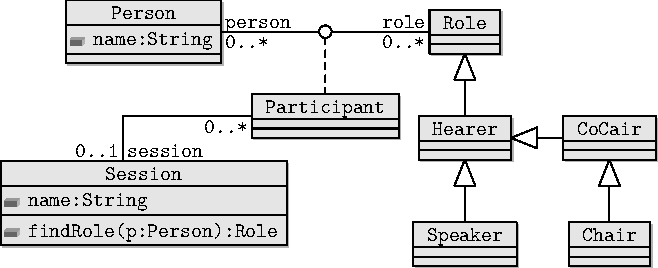
\includegraphics{figures/AbstractSimpleChair}}%
  \caption{A simple \UML class model representing a conference
    system for organizing conference sessions: persons can
    participate, in different roles, in a session. \label{fig:uml}}
\end{figure*}
One of the more prominent model types of the \UML is the
\emph{class model} (visualized as \emph{class diagram}) for modeling
the underlying data model of a system in an object-oriented manner. As
a running example, we model a part of a conference management
system. Such a system usually supports the conference organizing
process, \eg, creating a conference Website, reviewing submissions,
registering attendees, organizing the different sessions and tracks,
and indexing and producing the resulting proceedings. In this example,
we constrain ourselves to the process of organizing conference
sessions; \autoref{fig:uml} shows the class model.  We model the
hierarchy of roles of our system as a hierarchy of classes (\eg,
\inlineocl{Hearer}, \inlineocl{Speaker}, or \inlineocl{Chair}) using
an \emph{inheritance} relation (also called \emph{generalization}). In
particular, \emph{inheritance} establishes a \emph{subtyping}
relationship, \ie, every \inlineocl{Speaker} (\emph{subclass}) is also
a \inlineocl{Hearer} (\emph{superclass}).

A class does not only describe a set of \emph{instances} (called
\emph{objects}), \ie, record-like data consisting of \emph{attributes}
such as \inlineocl{name} of class \inlineocl{Session}, but also
\emph{operations} defined over them. For example, for the class
\inlineocl{Session}, representing a conference session, we model an
operation \inlineocl{findRole(p:Person):Role} that should return the
role of a \inlineocl{Person} in the context of a specific session;
later, we will describe the behavior of this operation in more detail
using \UML\@. In the following, the term object describes a
(run-time) instance of a class or one of its subclasses.

Relations between classes (called \emph{associations} in \UML)
can be represented in a class diagram by connecting lines, \eg,
\inlineocl{Participant} and \inlineocl{Session} or \inlineocl{Person}
and \inlineocl{Role}. Associations may be labeled by a particular
constraint called \emph{multiplicity}, \eg, \inlineocl+0..*+ or
\inlineocl+0..1+, which means that in a relation between participants
and sessions, each \inlineocl{Participant} object is associated to at
most one \inlineocl{Session} object, while each \inlineocl{Session}
object may be associated to arbitrarily many \inlineocl{Participant}
objects. Furthermore, associations may be labeled by projection
functions like \inlineocl{person} and \inlineocl{role}; these implicit
function definitions allow for \OCL-expressions like
\inlineocl+self.person+, where \inlineocl+self+ is a variable of the
class \inlineocl{Role}. The expression \inlineocl+self.person+ denotes
persons being related to the specific object \inlineocl{self} of
type role. A particular feature of the \UML are \emph{association
  classes} (\inlineocl{Participant} in our example) which represent a
concrete tuple of the relation within a system state as an object;
\ie, associations classes allow also for defining attributes and
operations for such tuples. In a class diagram, association classes
are represented by a dotted line connecting the class with the
association. Associations classes can take part in other associations.
Moreover, \UML supports also $n$-ary associations (not shown in
our example).

We refine this data model using the Object Constraint Language (\OCL)
for specifying additional invariants, preconditions and postconditions
of operations. For example, we specify that objects of the class
\inlineocl{Person} are uniquely determined by the value of the
\inlineocl{name} attribute and that the attribute \inlineocl{name} is
not equal to the empty string (denoted by \inlineocl{''}):
\begin{ocl}
context Person
  inv: name <> '' and
       Person::allInstances()->isUnique(p:Person | p.name)
\end{ocl}
Moreover, we specify that every session has exactly one chair by the
following invariant (called \inlineocl{onlyOneChair}) of the class
\inlineocl{Session}:
\begin{ocl}
context Session
  inv onlyOneChair: self.participants->one( p:Participant |
                                      p.role.oclIsTypeOf(Chair))
\end{ocl}
where \inlineocl{p.role.oclIsTypeOf(Chair)} evaluates to true, if
\inlineocl{p.role} is of \emph{dynamic type}
\inlineocl{Chair}. Besides the usual \emph{static types} (\ie, the
types inferred by a static type inference), objects in \UML and other
object-oriented languages have a second \emph{dynamic} type concept.
This is a consequence of a family of \emph{casting functions} (written
$\typeCast{o}{C}$ for an object $o$ into another class type $C$) that
allows for converting the static type of objects along the class
hierarchy. The dynamic type of an object can be understood as its
``initial static type'' and is unchanged by casts. We complete our
example by describing the behavior of the operation
\inlineocl{findRole} as follows:
\begin{ocl}
context Session::findRole(person:Person):Role
  pre:  self.participates.person->includes(person)
  post: result=self.participants->one(p:Participant |
                                p.person = person ).role
        and self.participants = self.participants@pre
        and self.name = self.name@pre
\end{ocl}
where in post-conditions, the operator \inlineocl{@pre} allows for
accessing the previous state.

In \UML, classes can contain attributes of the type of the
defining class.  Thus, \UML can represent (mutually) recursive
datatypes. Moreover, \OCL introduces also recursively specified
operations.

A key idea of defining the semantics of \UML and extensions like
Secure\UML~\cite{brucker.ea:transformation:2006} is to translate the
diagrammatic \UML features into a combination of more elementary
features of \UML and \OCL
expressions~\cite{gogolla.ea:expressing:2001}. For example,
associations are usually represented by collection-valued class
attributes together with \OCL constraints expressing the
multiplicity. Thus, having a semantics for a subset of \UML and \OCL is
tantamount for the foundation of the entire method.



\section{Formal Foundation}


\subsection{Isabelle}
Isabelle~\cite{nipkow.ea:isabelle:2002} is a \emph{generic} theorem
prover. New object logics can be introduced by specifying their syntax
and natural deduction inference rules. Among other logics, Isabelle
supports first-order logic, Zermelo-Fraenkel set theory and the
instance for Church's higher-order logic (HOL).

Isabelle's inference rules are based on the built-in meta-level
implication $\_ \Implies \_$ allowing to form constructs like $A_1
\Implies \cdots \Implies A_n \Implies A_{n+1}$, which are viewed as a
\emph{rule} of the form ``from assumptions $A_1$ to $A_n$, infer
conclusion $A_{n+1}$'' and which is written in Isabelle as
\begin{gather}
  \semantics{A_1 ; \ldots; A_n}\Implies A_{n+1}
  \qquad
  \text{or, in mathematical notation,}
  \quad
  \begin{prooftree}
    A_1 \qquad \cdots \qquad A_n
    \justifies
    A_{n+1}
    \ptmi{.}
  \end{prooftree}
\end{gather}
The built-in meta-level quantification $\Forall x\spot  x$ captures
the usual side-constraints ``$x$ must not occur free in the
assumptions'' for quantifier rules; meta-quantified variables can be
considered as ``fresh'' free variables. Meta-level quantification
leads to a generalization of Horn-clauses of the form:
\begin{gather}
\Forall x_1, \ldots, x_m\spot \semantics{A_1 ; \ldots; A_n}\Implies
A_{n+1}\mi{.}
\end{gather}

Isabelle supports forward- and backward reasoning on rules.  For
backward-reasoning, a \emph{proof-state} can be initialized and
further transformed into others. For example, a proof of $\phi$, using
the Isar~\cite{wenzel:isabelleisar:2002} language, will look as
follows in Isabelle:
\begin{gather}
  \begin{array}{l}
    \Lemma{label} \phi\\
    \quad\apply{case\_tac}\\
    \quad\apply{simp\_all}\\
  \done
  \end{array}
\end{gather}
This proof script instructs Isabelle to prove $\phi$ by case
distinction followed by a simplification of the resulting proof state.
Such a proof state is an implicitly conjoint sequence of generalized
Horn-clauses (called \emph{subgoals}) $\phi_1$, \ldots,$\phi_n$ and a
\emph{goal} $\phi$. Proof states were usually denoted by:
\begin{gather}
\begin{array}{rl}
\pglabel{label}:& \phi \\
 1.& \phi_1 \\
    &\vdots \\
 n.& \phi_n\\
\end{array}
\end{gather}
Subgoals and goals may be extracted from the proof state into theorems
of the form $\semantics{\phi_1 ; \ldots; \phi_n}\Implies \phi$ at any
time; this mechanism helps to generate test theorems.  Further,
Isabelle supports meta-variables (written $\meta{x}, \meta{y},
\ldots$), which can be seen as ``holes in a term'' that can still be
substituted. Meta-variables are instantiated by Isabelle's built-in
higher-order unification.

\subsection{Higher-order Logic (HOL)}
\emph{Higher-order logic}
(HOL)~\cite{church:types:1940,andrews:introduction:2002} is a
classical logic based on a simple type system.  It provides the usual
logical connectives like $\_ \land \_$, $\_ \implies\_$, $\lnot \_ $
as well as the object-logical quantifiers $\forall x\spot P\ap x$ and
$\exists x\spot P\ap x$; in contrast to first-order logic, quantifiers
may range over arbitrary types, including total functions
$f\ofType\alpha \Rightarrow \beta$. HOL is centered around
extensional equality $\_ = \_ \ofType \alpha \Rightarrow \alpha
\Rightarrow \text{bool}$.  HOL is more expressive than first-order
logic, since, \eg, induction schemes can be expressed inside the
logic. Being based on some polymorphically typed $\lambda$-calculus,
HOL can be viewed as a combination of a programming language
like SML or Haskell and a specification language providing
powerful logical quantifiers ranging over elementary and function
types.

Isabelle/HOL is a logical embedding of HOL into Isabelle.  The
(original) simple-type system underlying HOL has been extended by
Hindley-Milner style polymorphism with type-classes similar to
Haskell.  While Isabelle/HOL is usually seen as proof assistant, we
use it as symbolic computation environment. Implementations on top of
Isabelle/HOL can re-use existing powerful deduction mechanisms such as
higher-order resolution, tableaux-based reasoners, rewriting
procedures, Presburger arithmetic, and via various integration
mechanisms, also external provers such as
Vampire~\cite{riazanov.ea:vampire:1999} and the SMT-solver
Z3~\cite{moura.ea:z3:2008}.

Isabelle/HOL offers support for a particular methodology to extend
given theories in a logically safe way: A theory-extension is
\emph{conservative} if the extended theory is consistent provided that
the original theory was consistent.  Conservative extensions can be
\emph{constant definitions}, \emph{type definitions}, \emph{datatype
  definitions}, \emph{primitive recursive definitions} and
\emph{wellfounded recursive definitions}.

For instance, the library includes the type constructor $\up{\tau} :=
\isasymbottom ~ | ~ \lift{\_} : \alpha$ that assigns to each type
$\tau$ a type $\up{\tau}$ \emph{disjointly extended} by the
exceptional element $\isasymbottom$. The function $\drop{\_} :
\up{\alpha} \to \alpha$ is the inverse of $\lift{\_}$ (unspecified for
$\isasymbottom$). Partial functions $\alpha \isasymrightharpoonup
\beta$ are defined as functions $\alpha \isasymRightarrow \up{\beta}$
supporting the usual concepts of domain ($\dom\;\_$) and range
($\ran\;\_$).

As another example of a conservative extension, typed sets were built
in the Isabelle libraries conservatively on top of the kernel of HOL
as functions to $\HolBoolean$; consequently, the constant definitions
for membership is as follows:\footnote{To increase readability, we use
  a slightly simplified presentation.}
\begin{gather}
  \begin{array}{lrll}
    \types& \alpha \HolSet            &= \alpha \Rightarrow \HolBoolean\\[.5ex]
    \definitionS &\operatorname{Collect}&\ofType (\alpha \Rightarrow
     \HolBoolean) \Rightarrow \HolSet{\alpha}  &\qquad\text{--- set comprehension}\\
    \where &\operatorname{Collect}\ap S      &\equiv S\\[.5ex]
     \definitionS &\operatorname{member}           &\ofType \alpha \Rightarrow
     \alpha \Rightarrow \HolBoolean &\qquad\text{---
       membership test}\\
     \where &\operatorname{member}\ap s\ap S &\equiv S s\\
  \end{array}
\end{gather}
Isabelle's syntax engine is instructed to accept the notation
$\{x \mid P\}$ for $\operatorname{Collect}\ap\lambda x\spot P$ and the
notation $s \in S$ for $\operatorname{member}\ap s\ap S$. As can be
inferred from the example, constant definitions are axioms that
introduce a fresh constant symbol by some closed, non-recursive
expressions; this type of axiom is logically safe since it works
like an abbreviation. The syntactic side conditions of this axiom are
mechanically checked, of course. It is straightforward to express the
usual operations on sets like $\_ \cup \_,
\_\cap\_\ofType\HolSet{\alpha} \Rightarrow \HolSet{\alpha} \Rightarrow
\HolSet{\alpha}$ as conservative extensions, too, while the rules of
typed set theory were derived by proofs from these definitions.

Similarly, a logical compiler is invoked for the following statements introducing
the types option and list:
\begin{gather}
  \begin{array}{lrll}
    \datatype & \HolOption       &= \HolNone \mid \HolSome{\alpha}\\[.5ex]
    \datatype & \HolList{\alpha} &= \operatorname{Nil} \mid
    \operatorname{Cons}\ap a\ap l
  \end{array}
\end{gather}
Here, $[]$ or $a\#l$ are an alternative syntax for $\operatorname{Nil}$
or $\operatorname{Cons}\ap a ~l$; moreover, $[a, b, c]$ is defined as
alternative syntax for $a\#b\#c\#[]$. These (recursive) statements
were internally represented in by internal type and constant
definitions. Besides the \emph{constructors} $\HolNone$, $\HolSome$,
$[]$ and $\operatorname{Cons}$, there is the match operation
\begin{gather}
\HolCase\ap x\ap\HolOf~\HolNone \isasymRightarrow F\ap \mid
\HolSome{a} \isasymRightarrow G\ap a
\end{gather}
respectively
\begin{gather}
\HolCase\ap x\ap\HolOf~[] \isasymRightarrow F\ap \mid \operatorname{Cons}\ap a\ap
r \isasymRightarrow G\ap a\ap r\mi{.}
\end{gather}
From the internal definitions (not shown here) several properties were
automatically derived. We show only the case for lists:
\begin{gather}\label{eq:datatype-rules}
  \begin{array}{ll}
    (\HolCase\ap[]\ap\HolOf\ap[] \Rightarrow F  \ap | \ap  (a\#r) \Rightarrow
    G\ap a\ap r) = F &\\
    (\HolCase \ap  b\#t  \ap \HolOf  \ap [] \Rightarrow F  \ap  | \ap
    (a\#r) \Rightarrow G\ap a\ap r) = G~b~t &\\ %
    \mbox{}[] \neq a\#t    &\text{-- distinctness} \\
    \semantics{ a = [] \implies P ; \exists~x~t\spot  a = x\#t \implies P } \Longrightarrow P &\text{-- exhaust} \\
    \semantics{ P [] ; \forall~at\spot  P t \implies P (a\#t) } \Longrightarrow P x      &\text{-- induct}
  \end{array}
\end{gather}
Finally, there is a compiler for primitive and wellfounded recursive
function definitions. For example, we may define the
$\operatorname{sort}$ operation of our running test example by:
\begin{gather}\label{eq:sortdef}
  \begin{array}{lll}
    \fun
    &\enspace\operatorname{ins} & \ofType
    [\alpha\ofType\mathrm{linorder}, \HolList{\alpha}]
    \Rightarrow
    \HolList{\alpha}\\
    \where
    &\enspace \operatorname{ins}\ap x \ap  [\;] &= [x]\\
    &\enspace \operatorname{ins}\ap x \ap (y\#\mathit{ys})&=
    \HolIf x < y
    \HolThen x\#  y \# ys
    \HolElse y\#(\operatorname{ins} \ap x \ap ys)
 \end{array}\\
  \begin{array}{lll}
    \fun
    &\enspace\operatorname{sort} & \ofType
    \HolList{(\alpha\ofType\mathrm{linorder})}
    \Rightarrow
    \HolList{\alpha}\\
    \where
    &\enspace \operatorname{sort}\ap [\;] &= [\;]\\
    &\enspace \operatorname{sort} (x\#\mathit{xs})&=
    \operatorname{ins}\ap x\ap (\operatorname{sort}\ap xs)
   \end{array}
\end{gather}
The internal (non-recursive) constant definition for these operations
is quite involved; however, the logical compiler will finally derive
all the equations in the statements above from this definition and
make them available for automated simplification.

Thus, Isabelle/\HOL also provides a large collection of theories like
sets, lists, multisets, orderings, and various arithmetic theories
which only contain rules derived from conservative definitions. In
particular, Isabelle manages a set of \emph{executable types and
  operators}, \ie, types and operators for which a compilation to
SML, OCaml or Haskell is possible. Setups for arithmetic types
such as $\text{int}$ have been done; moreover any datatype and any
recursive function were included in this executable set (providing
that they only consist of executable operators). Similarly, Isabelle
manages a large set of (higher-order) rewrite rules into which
recursive function definitions were included. Provided that this
rule set represents a terminating and confluent rewrite system, the
Isabelle simplifier provides also a highly potent decision procedure
for many fragments of theories underlying the constraints to be
processed when constructing test theorems.

\section{How this Annex A was Generated from Isabelle/HOL Theories}
\fixme{Here ? Or in chap 2 ?}
\begin{figure*}[tb]
  \mbox{}\hfill
  \subfloat%
  [The Isabelle jEdit environment. ]%
  {\label{fig:jedit} 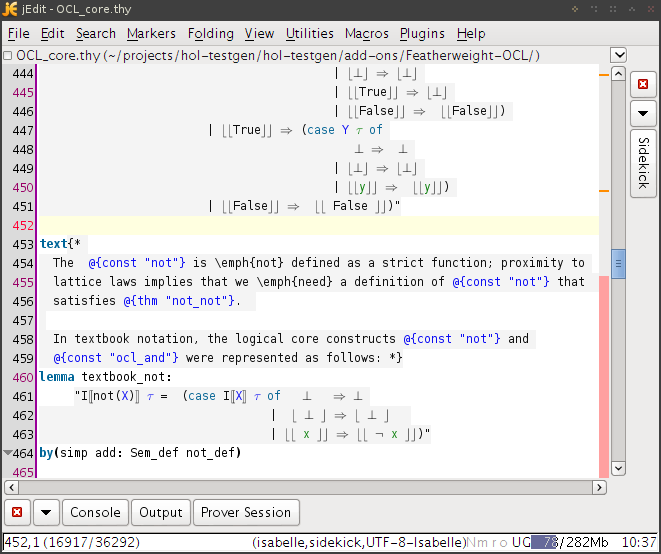
\includegraphics[height=6.2cm]{jedit}}%
  \hfill%
  \hfill%
    \subfloat[The generated formal document.]%
    {\label{fig:pdf} 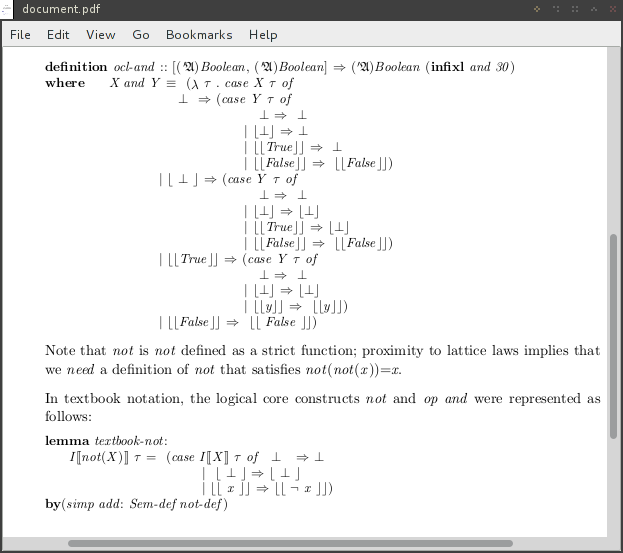
\includegraphics[height=6.2cm]{pdf}}
    \hfill\mbox{}
  \caption{Generating documents with guaranteed  syntactical and
    semantical consistency.}
  \label{fig:gener-docum-where}
\end{figure*}
Isabelle, as a framework for building formal
tools~\cite{wenzel.ea:building:2007}, provides the means for
generating \emph{formal documents}.  With formal documents (such as
the one you are currently reading) we refer to documents that are
machine-generated and ensure certain formal guarantees. In particular,
all formal content (\eg, definitions, formulae, types) are checked for
consistency during the document generation.

For writing documents, Isabelle supports the embedding of informal
texts using a \LaTeX-based markup language within the theory files. To
ensure the consistency, Isabelle supports to use, within these
informal texts, \emph{antiquotations} that refer to the formal parts
and that are checked while generating the actual document as
PDF\@. For example, in an informal text, the antiquotation
\inlineisar|@{$\text{thm}$ "not_not"}| will instruct Isabelle to
lock-up the (formally proven) theorem of name \inlineisar"ocl_not_not"
and to replace the antiquotation with the actual theorem, \ie,
\inlineocl{not (not x) $=$ x}.

\autoref{fig:gener-docum-where}
illustrates this approach: \autoref{fig:jedit} shows the jEdit-based
development environment of Isabelle with an excerpt of one of the core
theories of \FOCL\@. \autoref{fig:pdf} shows the generated
PDF document where all antiquotations are replaced. Moreover,
the document generation tools allows for defining syntactic sugar as
well as skipping technical details of the formalization.


Thus, applying the  \FOCL approach to writing an updated
Annex A that provides a formal semantics of the most fundamental
concepts of \OCL would ensure
\begin{enumerate}
\item that all formal context is syntactically correct and well-typed,
  and
\item all formal definitions and the derived logical rules are
  semantically consistent.
\end{enumerate}
Overall, this would contribute to one of the main goals of the \OCL 2.5
RFP, as discussed at the \OCL meeting in
Aachen~\cite{brucker.ea:summary-aachen:2013}.



\chapter{The Essence of UML-OCL Semantics}
\fixme{Generate this chapter from Isabelle theories ? Just for principle ?}
\section{The Theory Organization}
The semantic theory is organized in a quite conventional manner in
three layers. The first layer, called the \emph{denotational
  semantics} comprises a set of definitions of the operators of the
language.  Presented as \emph{definitional axioms} inside
Isabelle/\HOL, this part assures the logically consistency of the
overall construction. The denotational definitions of types, constants
and operations, and \OCL contracts represent the ``gold standard'' of the
semantics. The second layer, called \emph{logical layer},
is derived from the former and centered around the notion of validity
of an \OCL formula $P$ for a state-transition from pre-state $\sigma$
to post-state $\sigma'$, validity statements were written $(\sigma,
\sigma') \models P$. Its major purpose is to logically establish facts
(lemmas and theorems) about the denotational definitions.
The third layer, called \emph{algebraic layer},
also derived from the former layers, tries to establish algebraic laws
of the form $P = P'$; such laws are amenable to equational reasoning
and also help for automated reasoning and code-generation. For an
implementor of an \OCL compiler, these consequences are of most interest.

For space reasons, we will restrict ourselves in this paper to a few
operators and make a traversal through all three layers to give a
high-level description of our formalization.  Especially, the details
of the semantic construction for sets and the handling of objects and
object universes were excluded from a presentation here.

\subsection{Denotational Semantics of Types}
The syntactic material for type expressions, called $\text{TYPES}(C)$, is inductively
defined as follows:
\begin{itemize}
\item $C \subseteq \text{TYPES}(C)$ 
\item $\text{Boolean}$, $\text{Integer}$, $\text{Real}$, $\text{Void}$, ... are elements
      of $\text{TYPES}(C)$
\item $\text{Sequence}(X)$, $\text{Set}(X)$, et $\text{Pair}(X,Y)$ (as example for a Tuple-type)
      are in  $\text{TYPES}(C)$ (if $X, Y \in \text{TYPES}(C)$).
\end{itemize}

Types were directly represented in \FOCL by types in \HOL; consequently,
any \FOCL type must provide elements for a bottom element (also denoted $\bot$) 
and a null element; this is achieved in Isabelle by a type-class $\TCnull$ that 
contains two distinguishable elements $\HolBot$ and $\HolNull$ (see \autoref{sec:focl-types}
  for the details of the construction).

Moreover, the representation mapping from \OCL types to \FOCL id 
one-to-one (\ie{} injective), and the corresponding \FOCL types were
constructed to represent \emph{exactly} the elements (``no junk, no confucion
  elements'') of their \OCL counterparts. The corresponding \FOCL types were
constructed in two stages: First, a \emph{base-type} is constructed whose
carrier set contains exactly the elements of the \OCL type. Secondly, this
base type is lifted to a \emph{valuation} type that we use for type-checking
\FOCL constants, operations, and expressions. The valuation type takes into account
that some \UML-\OCL functions of its \OCL type (namely: accessors in path-expressions)
depend on a pre- and a post-state.

For most base types like $\text{Boolean}_{\text{base}}$ or $\text{Integer}_{\text{base}}$, it suffices 
to double-lift a \HOL library type:
\begin{equation*}
\typedef \qquad  \text{Boolean}_{\text{base}} \equiv \up{{\up{bool}}}
\end{equation*}
\fixme{Replace by typesynonym}
As a consequence of this type synonym, we have the elements $\HolBot, \lift{\HolBot}, 
\lift{\lift{\HolTrue}},\lift{\lift{\HolFalse}}$ in the carrier-set of  $\text{Boolean}_{\text{base}}$.
For object base types, we assume a typed universe $\Alpha$ of objects to be discussed later,
for the moment we will refer it by its polymorphic variable. 

With respect the valuation types for \OCL expression in general and Boolean expressions in
particular, they depend on the pair $(\sigma, \sigma')$ of pre-and post-state.  
Thus, we define valuation types by the synonym:
\begin{equation*}
  \V{\Alpha}{\alpha} \defeq \state{\Alpha} \times \state{\Alpha} \to \alpha \ofType \TCnull \mi{.}
\end{equation*}

The rules of the logical layer (there are no algebraic rules for the semantic sections on types),
and more details can be found in  \autoref{sec:focl-types}.

\subsection{Denotational Semantics of Constants and Operations}
We use the notation $I\semantics{E}$ for the semantic interpretation function as
commonly used in mathematical textbooks and the variable $\tau$ standing for pairs of
pre- and post state $(\sigma, \sigma')$. For reasons of conciseness,
we will write $\delta~X$ for $\mocl{not}\;X\mocl{.oclIsUndefined()}$
and $\upsilon~X$ for $\mocl{not}\;X\mocl{.oclIsInvalid()}$ throughout
this paper.
\begin{gather*}
\begin{alignedat}{3}
I\semantics{\mocl{invalid}\ofType V(\alpha)} \tau &\equiv \HolBot &
\qquad I\semantics{\mocl{null}\ofType V(\alpha)}  \tau    &\equiv \HolNull\\
I\semantics{\mocl{true}\ofType\mocl{Boolean}} \tau &=\lfloor\lfloor
\HolTrue\rfloor\rfloor &
I\semantics{\mocl{false}} \tau &= \lfloor\lfloor\HolFalse\rfloor\rfloor\\
\end{alignedat}\\
I\semantics{X\mocl{.oclIsUndefined()}} \tau =
    (\HolIf I\semantics{X}\tau \in \{\HolBot, \HolNull\} \HolThen I\semantics{\mocl{true}}\tau \HolElse I\semantics{\mocl{false}}\tau)\\
 I\semantics{X\mocl{.oclIsInvalid()}} \tau =
    (\HolIf I\semantics{X}\tau = \HolBot \HolThen I\semantics{\mocl{true}}\tau \HolElse I\semantics{\mocl{false}}\tau)
\end{gather*}

Due to the used style of
semantic representation (a shallow embedding) $I$ is in fact
superfluous and defined semantically as the identity; instead of:
\begin{gather*}
I\semantics{\mocl{true}\ofType\mocl{Boolean}} \tau =\lfloor\lfloor \HolTrue\rfloor\rfloor
\shortintertext{we can therefore write:}
\mocl{true}\ofType\mocl{Boolean}  = \lambda \tau. \lfloor\lfloor
\HolTrue\rfloor\rfloor
\end{gather*}
In Isabelle theories, this particular presentation of definitions
paves the way for an automatic check that the underlying equation
has the form of an \emph{axiomatic
definition} and is therefore logically safe.
Since all operators of the assertion language depend on the context $\tau$ = $(\sigma,
\sigma')$ and result in values that can be $\isasymbottom$, all expressions can
be viewed as \emph{evaluations} from $(\sigma, \sigma')$ to a type $\alpha$
which must posses a $\bottom$ and a $\text{null}$-element. Given that such
constraints can be expressed in Isabelle/HOL via \emph{type classes} (written: $\alpha::\kappa$),
all types for \OCL-expressions are of a form captured by
\begin{equation*}
 \V{}{\alpha} \defeq \state{} \times \state{} \to \alpha::\{bot,null\}  \mi{,}
 \end{equation*}
where $\state{}$ stands for the system state and $\state{} \times
\state{}$ describes the pair of pre-state and post-state and
$\_\defeq\_$ denotes the type abbreviation.

The current \OCL semantics~\cite[Annex A]{omg:ocl:2003} uses different
interpretation functions for invariants and pre-conditions; we achieve
their semantic effect by a syntactic transformation $\__\text{pre}$
which replaces, for example, all accessor functions
$\getAttrib{\_}{a}$ by their counterparts
$\getAttrib{\_}{a\isasymOclATpre}$. For example,
$(\getAttrib{\self}{a} > 5)_\text{pre}$ is just
$(\getAttrib{\self}{a\isasymOclATpre} > 5)$. This way, also invariants
and pre-conditions can be interpreted by the same interpretation
function and have the same type of an evaluation $\V{}{\alpha}$.


On this basis, one can define the core logical operators $\mocl{not}$
and $\mocl{and}$ as follows:
\begin{gather*}
  \begin{array}{ll}
    I\semantics{\mocl{not}\; X}  \tau
    &=  (\HolCase I\semantics{X} \tau  \HolOf\\
    &\quad\begin{array}{ll}
                     ~ \bottom                    &\Rightarrow  \bottom \\
                     | \lfloor  \bottom  \rfloor  &\Rightarrow  \lfloor  \bottom  \rfloor  \\
                     | \lfloor \lfloor  x \rfloor \rfloor  &\Rightarrow  \lfloor \lfloor  \lnot  x \rfloor \rfloor )
          \end{array}
  \end{array}
\end{gather*}

\begin{gather*}
  \begin{array}{ll}
   I\semantics{X\;\mocl{and}\; Y}  \tau
    &=  (\HolCase I\semantics{X} \tau  \HolOf\\
    &\quad\begin{array}{ll}
      ~ \bottom                    &\Rightarrow
      (\HolCase I\semantics{Y} \tau  \HolOf\\
      &\quad\begin{array}{ll}
                     ~ \bottom                    &\Rightarrow  \bottom \\
                     | \lfloor  \bottom  \rfloor  &\Rightarrow  \bottom  \\
                     | \lfloor \lfloor  \HolTrue \rfloor \rfloor
                     &\Rightarrow  \bottom\\
                     | \lfloor \lfloor  \HolFalse \rfloor \rfloor
                     &\Rightarrow  \lfloor \lfloor  \HolFalse \rfloor \rfloor )\\
                   \end{array}
      \\
                     | \lfloor  \bottom  \rfloor  &\Rightarrow
      (\HolCase I\semantics{Y} \tau  \HolOf\\
      &\quad\begin{array}{ll}
                     ~ \bottom                    &\Rightarrow
                     \bottom \\
                     | \lfloor  \bottom  \rfloor  &\Rightarrow  \lfloor
                     \bottom \rfloor \\
                     | \lfloor \lfloor  \HolTrue \rfloor \rfloor
                     &\Rightarrow  \lfloor \bottom\rfloor\\
                     | \lfloor \lfloor  \HolFalse \rfloor \rfloor
                     &\Rightarrow  \lfloor \lfloor  \HolFalse \rfloor \rfloor )\\
                   \end{array}
      \\
                     | \lfloor \lfloor  \HolTrue \rfloor \rfloor  &\Rightarrow
      (\HolCase I\semantics{Y} \tau  \HolOf\\
      &\quad\begin{array}{ll}
                     ~ \bottom                    &\Rightarrow
                     \bottom \\
                     | \lfloor  \bottom  \rfloor  &\Rightarrow  \lfloor
                     \bottom \rfloor \\
                     | \lfloor \lfloor y \rfloor \rfloor
                     &\Rightarrow  \lfloor \lfloor  y \rfloor \rfloor )\\
                   \end{array}
      \\
                     | \lfloor \lfloor  \HolFalse \rfloor \rfloor
                     &\Rightarrow   \lfloor \lfloor  \HolFalse \rfloor
                     \rfloor )\\
                   \end{array}\\
\end{array}
\end{gather*}
These non-strict operations were used to define the other logical connectives in the
usual classical way: $X\; \mocl{or}\; Y \equiv (\mocl{not}\; X)\;
\mocl{and}\; (\mocl{not}\; Y)$ or
$X\;\mocl{implies}\;Y \equiv (\mocl{not}\; X)\;\mocl{or}\; Y$.

The default semantics for an \OCL library operator is strict
semantics; this means that the result of an operation $f$ is
\inlineisar+invalid+ if one of its arguments is \inlineisar+invalid+.
For a semantics comprising \inlineisar+null+, we suggest to stay
conform to the standard and define the addition for integers as
follows:
 \begin{gather*}
   \begin{array}{rl}
   I\semantics{x \;\mocl{+}\; y}\tau  = &\HolIf I\semantics{\delta ~ x}\tau =\lfloor \lfloor \HolTrue\rfloor \rfloor  \land   I\semantics{\delta  ~ y}\tau =\lfloor \lfloor \HolTrue\rfloor \rfloor \\
                &\HolThen \lfloor \lfloor \lceil \lceil I\semantics{x}\tau \rceil \rceil  + \lceil \lceil I\semantics{y}\tau \rceil \rceil \rfloor \rfloor\\
                &\HolElse \bottom
   \end{array}
 \end{gather*}
 where the operator ``\mocl{+}'' on the left-hand
 side of the equation denotes the \OCL addition of type
 $[\V{}{\up{(\up{\HolInteger})}}, \V{}{\up{(\up{\HolInteger})}}] \Rightarrow
 \V{}{\up{(\up{\HolInteger})}}$ while the ``$+$'' on the right-hand side of
 the equation of type $[\HolInteger,\HolInteger]\Rightarrow
 \HolInteger$ denotes the integer-addition from the HOL library.

\subsection{Logical Layer}
The topmost goal of the logic for \OCL is to define the \emph{validity statement}:
\begin{equation*}
   (\sigma, \sigma') \isasymMathOclValid P\mi{,}
\end{equation*}
where $\sigma$ is the pre-state and $\sigma'$ the post-state of the
underlying system and $P$ is a formula.
Informally, a formula $P$ is valid if and only if its evaluation in
$(\sigma, \sigma')$ (\ie, $\tau$ for short) yields true. Formally this means:
\begin{equation*}
\tau \isasymMathOclValid P \equiv \bigl(I\semantics{P} \tau =  \lfloor \lfloor \HolTrue  \rfloor \rfloor \bigr)\mi{.}
\end{equation*}
On this basis, classical, two-valued inference rules can be established for
reasoning over the logical connective, the different notions of equality,
definedness and validity. Generally speaking, rules over logical validity can
relate bits and pieces in various \OCL terms and allow---via strong
logical equality discussed below---the replacement
of semantically equivalent sub-expressions. The core inference rules are:
\begin{gather*}
\begin{array}{lccr}
  \tau \models \mocl{true} &\quad
  \lnot(\tau \models \mocl{false})&\quad
  \lnot(\tau \models \mocl{invalid})&\quad
  \lnot(\tau \models \mocl{null})
\end{array}\\
  \tau \models \mocl{not}\; P \Longrightarrow \lnot (\tau \models P)\\
\begin{array}{lcr}
  \tau \models P \;\mocl{and}\; Q \Longrightarrow \tau \models P&\qquad&
  \tau \models P \;\mocl{and}\; Q \Longrightarrow \tau \models Q
\end{array}\\
  \tau \models P \Longrightarrow
     (\mocl{if}\; P \;\mocl{then}\; B_1 \;\mocl{else}\; B_2 \;\mocl{endif})\tau = B_1\ap \tau\\
  \tau \models \mocl{not}\; P \Longrightarrow
       (\mocl{if}\; P \;\mocl{then}\; B_1 \;\mocl{else}\; B_2 \;\mocl{endif})\tau = B_2\ap \tau\\
\begin{array}[lcr]{lcr}
  \tau \models P \Longrightarrow \tau \models \delta \ap P &\qquad&
  \tau \models \delta \ap X \Longrightarrow \tau \models \upsilon \ap X
\end{array}
\end{gather*}
By the latter two properties it can be inferred that any valid
property $P$ (so for example: a valid invariant) is defined, which
allows to infer for terms composed by strict operations that their
arguments and finally the variables occurring in it are valid or
defined.

We propose to distinguish the \emph{strong logical equality} (written
$\_ \isasymMathOclStrongEq \_$), which follows the general principle
that ``equals can be replaced by equals,'' from the \emph{strict
  referential equality} (written $\_ \isasymMathOclStrictEq \_$),
which is an object-oriented concept that attempts to approximate and
to implement the former.  Strict referential equality, which is the
default in the \OCL language and is written \inlineocl|_ = _|
in the standard, is an overloaded concept and has to be defined for
each \OCL type individually; for objects resulting from class
definitions, it is implemented by comparing the references to
the objects. In contrast, strong logical equality is a polymorphic
concept which is defined once and for all by:
\begin{gather*}
  I\semantics{X \triangleq  Y}  \tau  \equiv  \lfloor \lfloor
  I\semantics{X}  \tau=
  I\semantics{Y} \tau  \rfloor \rfloor
\shortintertext{It enjoys nearly the laws of a congruence:}
\tau \models (x \triangleq x)\\
\tau \models (x \triangleq y) \Longrightarrow \tau \models (y \triangleq x)\\
\tau \models (x \triangleq y) \Longrightarrow \tau \models (y \triangleq z) \Longrightarrow \tau \models (x \triangleq z)\\
\HolOclCp P \Longrightarrow \tau \models (x \triangleq y) \Longrightarrow \tau \models (P\ap x) \Longrightarrow \tau \models (P\ap y)
\end{gather*}
where the predicate $\HolOclCp$ stands for \emph{context-passing}, a
property that is characterized by $P(X)$ equals $\lambda \tau\spot
P(\lambda \_\spot X \tau) \tau$. It means that the state tuple $\tau =
(\sigma, \sigma')$ is passed unchanged from surrounding expressions to
sub-expressions. it is true for all pure \OCL expressions (but not
arbitrary mixtures of \OCL and HOL) in \FOCL\@.  The
necessary side-calculus for establishing $\HolOclCp$ can be fully
automated.

The logical layer of the  \FOCL rules gives also a means
to convert an \OCL formula living in its four-valued world into a
representation that is classically two-valued and can be processed by
standard SMT solvers such as CVC3~\cite{barrett.ea:cvc3:2007} or
Z3~\cite{moura.ea:z3:2008}. $\delta$-closure rules for all logical
connectives have the following format, \eg:
\begin{gather*}
\tau \models \delta \ap x \Longrightarrow (\tau \models \ap\mocl{not}\ap x) = (\lnot (\tau \models x))\\
\tau \models \delta \ap x \Longrightarrow \tau \models \delta \ap y \Longrightarrow (\tau \models x \ap\mocl{and}\ap y) = ( \tau \models x \land \tau \models y)\\
\begin{multlined}
\tau \models \delta \ap x \Longrightarrow  \tau \models \delta \ap y \\
\Longrightarrow (\tau \models (x \ap\mocl{implies}\ap y)) = ( (\tau \models x) \longrightarrow (\tau \models y))
\end{multlined}
\end{gather*}
Together with the general case-distinction
\begin{gather*}
    \tau \models \delta \ap x \lor \tau \models x \triangleq \mocl{invalid} \lor \tau \models x \triangleq \mocl{null} \mi{,}
\end{gather*}
which is possible for any \OCL type, a case distinction on the
variables in a formula can be performed; due to strictness rules,
formulae containing somewhere a variable $x$ that is known to be
$\mocl{invalid}$ or $\mocl{null}$ reduce usually quickly to
contradictions.  For example, we can infer from an invariant $\tau
\models x \isasymMathOclStrictEq y \;\mocl{-}\; \mocl{3}$ that we have $\tau
\models x \isasymMathOclStrictEq y \;\mocl{-}\; \mocl{3} \land \tau \models
\delta \ap x \land \tau \models \delta \ap y$.  We call the latter formula the
$\delta$-closure of the former.  Now, we can convert a formula like
$\tau \models x \;\mocl{>}\; \mocl{0} \ap\mocl{or}\ap \mocl{3} \;\mocl{*}\; y \;\mocl{>}\;
x \;\mocl{*}\; x$ into the equivalent formula
$\tau \models x \;\mocl{>}\; \mocl{0} \lor \tau
\models \mocl{3} \;\mocl{*}\; y \;\mocl{>}\; x \;\mocl{*}\; x$ and thus internalize the
\OCL-logic into a classical (and more tool-conform) logic. This
works---for the price of a potential, but due to the usually ``rich''
$\delta$-closures of invariants rare---exponential blow-up of the
formula for all \OCL formulas.

\subsection{Algebraic Layer}
Based on the logical layer, we build a system with simpler rules which
are amenable to automated reasoning. We restrict ourselves to pure
equations on \OCL expressions, where the used equality is the
meta-(HOL-)equality.

Our denotational definitions on \inlineocl+not+ and \inlineocl+and+
can be re-formulated in the following ground equations:
\begin{gather*}
  \begin{aligned}
  \upsilon\; \mocl{invalid} &= \mocl{false}&\qquad
  \upsilon\; \mocl{null} &= \mocl{true}\\
  \upsilon\; \mocl{true} &= \mocl{true}&\qquad
  \upsilon\; \mocl{false} &= \mocl{true}\\
\end{aligned}\\[.04\baselineskip]
\begin{aligned}
  %
  \delta\; \mocl{invalid} &= \mocl{false}&\qquad
  \delta\; \mocl{null} &= \mocl{false}\\
  \delta\; \mocl{true} &= \mocl{true}&\qquad
  \delta\; \mocl{false} &= \mocl{true}\\
\end{aligned}\\[.04\baselineskip]
\begin{aligned}
  %
  \mocl{not}\; \mocl{invalid} &= \mocl{invalid}&\qquad
  \mocl{not}\; \mocl{null} &= \mocl{null}\\
  \mocl{not}\; \mocl{true} &= \mocl{false}&\qquad
  \mocl{not}\; \mocl{false} &= \mocl{true}\\
\end{aligned}\\[.04\baselineskip]
\begin{aligned}
  %
  (\mocl{null} \;\mocl{and}\; \mocl{true}) &= \mocl{null}&\qquad
  (\mocl{null} \;\mocl{and}\; \mocl{false}) &= \mocl{false}\\
  (\mocl{null} \;\mocl{and}\; \mocl{null}) &= \mocl{null}&\qquad
  (\mocl{null} \;\mocl{and}\; \mocl{invalid}) &= \mocl{invalid}\\
\end{aligned}\\[.04\baselineskip]
\begin{aligned}
  %
  (\mocl{false} \;\mocl{and}\; \mocl{true}) &= \mocl{false}&\qquad
  (\mocl{false} \;\mocl{and}\; \mocl{false}) &= \mocl{false}\\
  (\mocl{false} \;\mocl{and}\; \mocl{null}) &= \mocl{false}&\qquad
  (\mocl{false} \;\mocl{and}\; \mocl{invalid}) &= \mocl{false}\\
\end{aligned}\\[.04\baselineskip]
\begin{aligned}
  %
  (\mocl{true} \;\mocl{and}\; \mocl{true}) &= \mocl{true}&\qquad
  (\mocl{true} \;\mocl{and}\; \mocl{false}) &= \mocl{false}\\
  (\mocl{true} \;\mocl{and}\; \mocl{null}) &= \mocl{null}&\qquad
  (\mocl{true} \;\mocl{and}\; \mocl{invalid}) &= \mocl{invalid}
\end{aligned}\\[.04\baselineskip]
\begin{aligned}
  (\mocl{invalid} \;\mocl{and}\; \mocl{true}) &= \mocl{invalid} \\
  (\mocl{invalid} \;\mocl{and}\; \mocl{false}) &= \mocl{false}\\
  (\mocl{invalid} \;\mocl{and}\; \mocl{null}) &= \mocl{invalid} \\
  (\mocl{invalid} \;\mocl{and}\; \mocl{invalid}) &= \mocl{invalid}\\
\end{aligned}
\shortintertext{On this core, the structure of a conventional lattice arises:}
  \begin{aligned}
    X \;\mocl{and}\; X &= X        &\qquad     X \;\mocl{and}\; Y &= Y \;\mocl{and}\; X
  \end{aligned}\\
  \begin{aligned}
    \mocl{false} \;\mocl{and}\; X &= \mocl{false} &\qquad
    X \;\mocl{and}\; \mocl{false} &= \mocl{false}  \\
    \mocl{true} \;\mocl{and}\; X  &= X &\qquad
    X \;\mocl{and}\; \mocl{true} &= X
  \end{aligned}\\
  \begin{aligned}
             X \;\mocl{and}\; (Y \;\mocl{and}\; Z) &= X \;\mocl{and}\; Y \;\mocl{and}\; Z
  \end{aligned}
\end{gather*}
as well as the dual equalities for \inlineocl|_ or _| and the De Morgan
rules.  This wealth of algebraic properties makes the understanding of
the logic easier as well as automated analysis possible: it allows
for, for example, computing a DNF of invariant systems (by
clever term-rewriting techniques) which are a prerequisite for
$\delta$-closures.

The above equations explain the behavior for the most-important
non-strict operations. The clarification of the exceptional behaviors
is of key-importance for a semantic definition the standard and the
major deviation point from
\HOLOCL~\cite{brucker.ea:hol-ocl:2008,brucker.ea:hol-ocl-book:2006},
to  \FOCL as presented here.  The
standard expresses at many places that most operations are strict,
\ie, enjoy the properties (exemplary for \inlineocl|_ + _|):
\begin{gather*}
  \begin{aligned}
  \mocl{invalid}\;\mocl{+}\; X &= \mocl{invalid}&\qquad
  X \;\mocl{+}\; \mocl{invalid} &= \mocl{invalid}\\
  X \;\mocl{+}\; \mocl{null} &= \mocl{invalid}&\qquad
  \mocl{null} \;\mocl{+}\; X &= \mocl{invalid}
  \end{aligned}\\
  \mocl{null.oclAsType(}X\mocl{)} = \mocl{invalid}
\shortintertext{besides ``classical'' exceptional behavior:}
  \begin{aligned}
    \mocl{1} \;\mocl{/}\; \mocl{0} &= \mocl{invalid} \quad &\quad
    \mocl{1} \;\mocl{/}\; \mocl{null} &= \mocl{invalid}
  \end{aligned}\\
    \mocl{null->isEmpty()}=\mocl{true}
\end{gather*}

Moreover, there is also the proposal to use \inlineocl+null+ as a kind
of ``don't know'' value for all strict operations, not only in the
semantics of the logical connectives.  Expressed in algebraic
equations, this semantic alternative (this is \emph{not}
 \FOCL at present) would boil down to:
\begin{gather*}
  \begin{aligned}
    \mocl{invalid} \;\mocl{+}\; X &= \mocl{invalid} &\qquad
    X \;\mocl{+}\; \mocl{invalid} &= \mocl{invalid}\\
    X \;\mocl{+}\; \mocl{null} &= \mocl{null}&\qquad
    \mocl{null} \;\mocl{+}\; X &= \mocl{null}
  \end{aligned}\\
    \mocl{null.oclAsType(}X\mocl{)} = \mocl{null}\\
  \begin{aligned}
    \mocl{1} \;\mocl{/}\; \mocl{0} &= \mocl{invalid} \quad &\quad
    \mocl{1} \;\mocl{/}\; \mocl{null} &= \mocl{null}
  \end{aligned}\\
    \mocl{null->isEmpty()}=\mocl{null}
\end{gather*}

While this is logically perfectly possible, while it can be argued
that this semantics is ``intuitive'', and although we do not expect a
too heavy cost in deduction when computing $\delta$-closures, we
object that there are other, also ``intuitive'' interpretations that
are even more wide-spread: In classical spreadsheet programs, for
example, the semantics tends to interpret \inlineocl+null+
(representing empty cells in a sheet) as the neutral element of the
type, so \inlineocl{0} or the empty string, for example.\footnote{In
  spreadsheet programs the interpretation of \inlineisar+null+ varies
  from operation to operation; \eg, the \inlineocl+average+
  function treats \inlineocl+null+ as non-existing value and not as
  \inlineocl{0}.}  This semantic alternative (this is
\emph{not}  \FOCL at present) would yield:
\begin{gather*}
  \begin{aligned}
    \mocl{invalid} \;\mocl{+}\; X &= \mocl{invalid} &\qquad
    X \;\mocl{+}\; \mocl{invalid} &= \mocl{invalid}\\
    X \;\mocl{+}\; \mocl{null} &= X&\qquad
    \mocl{null} \;\mocl{+}\; X &= X
  \end{aligned}\\
    \mocl{null.oclAsType(}X\mocl{)} = \mocl{invalid}\\
  \begin{aligned}
    \mocl{1} \;\mocl{/}\; \mocl{0} &= \mocl{invalid} \quad &\quad
    \mocl{1} \;\mocl{/}\; \mocl{null} &= \mocl{invalid}
\end{aligned}\\
    \mocl{null->isEmpty()}=\mocl{true}
\end{gather*}

Algebraic rules are also the key for execution and compilation
of  \FOCL expressions. We derived, \eg:
\begin{gather*}
\delta\; \mocl{Set\{\}} = \mocl{true}\\
\delta\; (X\mocl{->including(}x\mocl{)}) = \delta \ap X \;\mocl{and}\;
 \upsilon \ap x\\
\begin{aligned}
\mocl{Set\{\}->includes(}x\mocl{)} = (\mocl{if}\; \upsilon\; x\; &\mocl{then false}\\
&\mocl{else invalid endif})
\end{aligned}\\
\begin{multlined}
  {(X\mocl{->including(}x\mocl{)->includes(}y\mocl{)})=}\\
  \mbox{\hspace{3.2cm}}\qquad{\begin{aligned}
   (&\mocl{if}\; \delta\; X\\
  &\mocl{then}\;
\begin{array}[t]{l}
\mocl{if}\; x \doteq y\\
\mocl{then}\ap \mocl{true} \\
\mocl{else}\ap X\mocl{->includes(}y\mocl{)}\\
\mocl{endif}
  \end{array}\\
&\mocl{else invalid} \\
         &\mocl{endif})
  \end{aligned}}
\end{multlined}
\end{gather*}
As \inlineocl+Set{1,2}+ is only syntactic sugar for
\begin{ocl}
  Set{}->including(1)->including(2)
\end{ocl}
an expression like \inlineocl+Set{1,2}->includes(null)+ becomes
decidable in  \FOCL by a combination of
rewriting and code-generation and execution. The generated
documentation from the theory files can thus be enriched by numerous
``test-statements'' like:
\begin{isar}[mathescape]
value  "\<tau> \<Turnstile> ($\mathtt{Set\{Set\{2,null\}\}}$ \<doteq> $\;\mathtt{Set\{Set\{null,2\}\}}$)"
\end{isar}
which have been machine-checked and which present a high-level and in
our opinion fairly readable information for \OCL tool manufactures and
users.


\section{Object-oriented Datatype Theories}
As mentioned earlier, the \OCL is composed of
\begin{enumerate}
\item operators on built-in data structures such as Boolean, Integer or Set(\_),
      and
\item operators of the user-defined data model such as accessors,
      type casts and tests.
\end{enumerate}

In the following, we will refine the concepts of a user-defined
data-model (implied by a \emph{class-model}, visualized by a class-diagram)
as well as the notion of $\state{}$ used in the
previous section to much more detail.  In contrast to wide-spread
opinions, \UML class models represent in a compact and visual manner
quite complex, object-oriented data-types with a surprisingly rich
theory. It is part of our endeavor here to make this theory explicit
and to point out corner cases.  A \UML class diagram---underlying a
given \OCL formula---produces several implicit operations which
become accessible via appropriate \OCL syntax:

\begin{enumerate}
\item Classes and class names (written as $C_1$, \ldots, $C_n$), which
  become types of data in \OCL\@. Class names declare two projector
  functions to the set of all objects in a state:
  $C_i$\inlineocl{.allInstances()} and
  $C_i$\inlineocl{.allInstances}$\isasymOclATpre$\inlineocl{()},
\item an inheritance relation $\_ < \_$ on classes, a collection of
  attributes $Attrib(C_i)$ associated to classes $C_i$,
  and a collection of associations $Assoc(C_i,C_j)$,
  \footnote{Given the fact that there is at present no consensus on the
  semantics of n-ary associations, \FOCL{} restricts itself to binary associations. }
\item two families of accessors; for each attribute $a \in Attrib(C_i) $ in a
  class definition $C_i$ (denoted
  $\getAttrib{X}{\text{$a$}}               :: C_i \rightarrow A $ and
  $\getAttrib{X}{\text{$a$}\isasymOclATpre}:: C_i \rightarrow A $ for
  $A\in \{\V{}{\up{\ldots}}, C_1, \ldots, C_n\}$),
\item An association $(n, rn_{from}, rn_{to})\in Assoc(C_i,C_j) $ between to classes 
      $C_i$ and $C_j$ is a triple consisting of a (unique) association name $n$, 
      and the rolenames $rn_{to}$ and $rn_{from}$. To each rolename belong two
      families of accessors   denoted
  $\getRole{X}{\text{$a$}}               :: C_i \rightarrow Collection(A) $ and
  $\getRole{X}{\text{$a$}\isasymOclATpre}:: C_i \rightarrow Colletion(A) $ for
  $A\in \{\V{}{\up{\ldots}}, C_1, \ldots, C_n\}$), 
\item type casts that can change the static type of an object of a
      class ($\getAttrib{X}{\mocl{oclAsType(}\text{$C_i$}\mocl{)}}$ of type
      $C_j \rightarrow C_i$)
\item two dynamic type tests ($\getAttrib{X}{\mocl{oclIsTypeOf(}\text{$C_i$}\mocl{)}}$ and
      $\getAttrib{X}{\mocl{oclIsKindOf(}\text{$C_i$}\mocl{)}}$ ),
\item and last but not least, for each class name $C_i$ there is an
  instance of the overloaded referential equality (written $\_
  \isasymMathOclStrictEq \_$).
\end{enumerate}


Assuming a strong static type discipline in the sense of
Hindley-Milner types,  \FOCL has no ``syntactic
subtyping.''  This does not mean that subtyping cannot be expressed
\emph{semantically} in  \FOCL; by giving a formal semantics
to type-casts, subtyping becomes an issue of the front-end that can
make implicit type-coersions explicit by introducing explicit
type-casts. Our perspective shifts the emphasis on the semantic
properties of casting, and the necessary universe of object
representations (induced by a class model) that allows to establish
them.


\subsection{Object Universes}

It is natural to construct system states by a set of partial functions
$f$ that map object identifiers $\oid$ to some representations of
objects:
\begin{gather}
       \typedef \qquad \alpha~\state{} \defeq \{ \sigma ::
        \oid \isasymrightharpoonup \alpha \ap|\ap \inv_\sigma(\sigma) \}
\end{gather}
where $\inv_\sigma$ is a to be discussed invariant on states.

The key point is that we need a common type $\alpha$ for the set of all
possible \emph{object representations}.  Object representations model
``a piece of typed memory,'' \ie, a kind of record comprising
administration information and the information for all attributes of
an object; here, the primitive types as well as collections over them
are stored directly in the object representations, class types and
collections over them are represented by $\oid$'s (respectively lifted
collections over them).

In a shallow embedding which must represent
\UML types injectively by HOL types, there are two fundamentally
different ways to construct such a set of object representations,
which we call an \emph{object universe} $\mathfrak{A}$:
\begin{enumerate}
\item an object universe can be constructed for a given class model,
  leading to \emph{closed world semantics}, and
\item an object universe can be constructed for a given class model
  \emph{and all its extensions by new classes added into the leaves of
    the class hierarchy}, leading to an \emph{open world semantics}.
\end{enumerate}
For the sake of simplicity, we chose the first option for
 \FOCL, while HOL-\OCL~\cite{brucker.ea:extensible:2008-b}
used an involved construction allowing the latter.

A na\"ive attempt to construct $\mathfrak{A}$ would look like this:
the class type $C_i$ induced by a class will be the type of such an
object representation: $C_i \defeq (\oid \times A_{i_1} \times \cdots
\times A_{i_k} )$ where the types $A_{i_1}$, \ldots, $A_{i_k}$ are the
attribute types (including inherited attributes) with class types
substituted by $\oid$. The function $\HolOclOidOf$ projects the first
component, the $\oid$, out of an object representation. Then the
object universe will be constructed by the type definition:
\begin{gather}
\mathfrak{A} := C_1 + \cdots +  C_n\mi{.}
\end{gather}
It is possible to define constructors, accessors, and the referential
equality on this object universe. However, the treatment of type casts
and type tests cannot be faithful with common object-oriented
semantics, be it in \UML or Java: casting up along the class hierarchy
can only be implemented by loosing information, such that casting up
and casting down will \emph{not} give the required identity:

\begin{gather}
        X.\mocl{oclIsTypeOf(}C_k\mocl{)} ~ ~  \mocl{implies} ~ ~ X\mocl{.oclAsType(}C_i\mocl{)}\mocl{.oclAsType(}C_k\mocl{)} \isasymMathOclStrictEq
   X \\
   \qquad \qquad  \qquad \qquad  \qquad \qquad \text{whenever $C_k  < C_i$ and $X$ is valid.}
\end{gather}


To overcome this limitation, we introduce an auxiliary type
$C_{i\text{ext}}$ for \emph{class type extension}; together, they were
inductively defined for a given class diagram:

Let $C_i$ be a class with a possibly empty set of subclasses
$\{C_{j_{1}}, \ldots, C_{j_{m}}\}$.
\begin{itemize}
\item Then the  \emph{class type extension} $C_{i\text{ext}}$
        associated to $C_i$ is
        $A_{i_{1}} \times \cdots \times A_{i_{n}} \times \up{(C_{j_{1}\text{ext}} + \cdots + C_{j_{m}\text{ext}})}$
        where $A_{i_{k}}$ ranges over the local
        attribute types of $C_i$ and $C_{j_{l}\text{ext}}$
        ranges over all class type extensions of the subclass $C_{j}$ of $C_i$.
\item Then the \emph{class type} for $C_i$ is
        $oid \times A_{i_{1}} \times \cdots \times A_{i_{n}} \times \up{(C_{j_{1}\text{ext}} + \cdots + C_{j_{m}\text{ext}})}$
        where $A_{i_{k}}$ ranges over the inherited \emph{and} local
        attribute types of $C_i$ and $C_{j_{l}\text{ext}}$
        ranges over all class type extensions of the subclass $C_{j}$ of $C_i$.
\end{itemize}

Example instances of this scheme---outlining a compiler---can be found
in \autoref{ex:employee-analysis:uml} and \autoref{ex:employee-design:uml}.

This construction can \emph{not} be done in HOL itself since it
involves quantifications and iterations over the ``set of class-types'';
rather, it is a meta-level construction.  Technically, this means that
we need a compiler to be done in SML on the syntactic
``meta-model''-level of a class model.

With respect to our semantic construction here,
which above all means is intended to be type-safe, this has the following consequences:
\begin{itemize}
\item there is a generic theory of states, which must be formulated independently
      from a concrete object universe,
\item there is a principle of translation (captured by the inductive scheme for
      class type extensions and class types above) that converts a given class model
      into an concrete object universe,
\item there are fixed principles that allow to derive the semantic theory of any
      concrete object universe, called the \emph{object-oriented datatype theory.}
\end{itemize}
We will work out concrete examples for the construction of the
object-universes in \autoref{ex:employee-analysis:uml} and \autoref{ex:employee-design:uml} and the
derivation of the respective datatype theories. While an
automatization is clearly possible and desirable for concrete
applications of  \FOCL, we consider this out of the scope
of this paper which has a focus on the semantic construction and its
presentation.


\subsection{Accessors on Objects and Associations}
Our choice to use a shallow embedding of \OCL in HOL and, thus having
an injective mapping from \OCL types to HOL types, results in
type-safety of  \FOCL\@. Arguments and results of accessors
are based on type-safe object representations and \emph{not} $\oid$'s.
This implies the following scheme for an accessor:
\begin{itemize}
\item The \emph{evaluation and extraction} phase. If the argument
  evaluation results in an object representation, the $\oid$ is
  extracted, if not, exceptional cases like \inlineocl{invalid} are
  reported.
\item The \emph{dereferentiation} phase. The $\oid$ is interpreted in
  the pre- or post-state, %(depending on the suffix of accessor),
  the resulting object is casted to the expected format.  The
  exceptional case of nonexistence in this state must be treated.
\item The \emph{selection} phase. The corresponding attribute is
  extracted from the object representation.
\item The \emph{re-construction} phase.  The resulting value has to be
  embedded in the adequate HOL type.  If an attribute has the type of
  an object (not value), it is represented by an optional (set of)
  $\oid$, which must be converted via dereferentiation in one of the
  states to produce an object representation again. The
  exceptional case of nonexistence in this state must be treated.
\end{itemize}

The first phase directly translates into the following formalization:
\begin{multline}
  \shoveleft{\definitionS}\quad\\
  \begin{array}{rllr}
 \operatorname{eval\_extract} X\ap f = (\lambda \tau\spot \HolCase
 X\ap
 \tau \HolOf & \bottom &\Rightarrow
 \mocl{invalid}\ap\tau&\text{exception}\\
 |& \lift{\bottom} &\Rightarrow
 \mocl{invalid}\ap\tau&\text{deref. null}\\
 |& \lift{\lift{\mathit{obj}}} &\Rightarrow f\ap (\operatorname{oid\_of} \ap \mathit{obj})\ap\tau)&
  \end{array}
\end{multline}

For each class $C$, we introduce the dereferentiation phase of this
form:
\begin{multline}
  \definitionS \ap
  \operatorname{deref\_oid}_C \ap \mathit{fst\_snd}\ap f\ap \mathit{oid} =
                     (\lambda \tau\spot \HolCase\ap (\operatorname{heap}\ap
                     (\mathit{fst\_snd}\ap \tau))\ap \mathit{oid}\ap
                     \HolOf\\
  \begin{array}{ll}
           \phantom{|}\ap \lift{\operatorname{in}_C obj} &\Rightarrow f\ap
                     \mathit{obj} \ap \tau\\
                     |\ap \_ &\Rightarrow \mocl{invalid}\ap \tau)
      \end{array}
   \end{multline}

The operation yields undefined if the $\oid$ is uninterpretable in the
state or referencing an object representation not conforming to the
expected type.

We turn to the selection phase: for each class $C$ in the class model
with at least one attribute,
and each attribute $a$ in this class,
we introduce the selection phase of this form:
\begin{gather}
  \begin{array}{rlcll}
  \definitionS \ap
    \operatorname{select}_a \ap f = (\lambda &
                  \operatorname{mk}_C \ap oid & \cdots \bottom \cdots & C_{X\text{ext}} & \Rightarrow \mocl{null}\\
                  |& \operatorname{mk}_C \ap oid & \cdots \lift{a} \cdots & C_{X\text{ext}}
                    &\Rightarrow f\ap (\lambda \ap x \ap \_\spot
                   \lift{\lift{x}})\ap a)
  \end{array}
\end{gather}

This works for definitions of basic values as well as for object
references in which the $a$ is of type $\oid$.  To increase
readability, we introduce the functions:
\begin{gather}
\begin{array}{llrlr}
\qquad\qquad&\definitionS\enspace&\operatorname{in\_pre\_state}    &= \operatorname{fst} & \qquad \text{first component}\\
\qquad\qquad&\definitionS\enspace&\operatorname{in\_post\_state}   &= \operatorname{snd} & \qquad \text{second component} \\
\qquad\qquad&\definitionS\enspace&\operatorname{reconst\_basetype} &= \operatorname{id} & \qquad \text{identity function}
\end{array}
\end{gather}


Let \_\inlineocl{.getBase} be an accessor of class $C$ yielding a
value of base-type $A_{base}$. Then its definition is of the form:
\begin{gather}
  \begin{array}{lll}
\definitionS&\_\mocl{.getBase} &\ofType \ap C \Rightarrow A_{base}\\
\where\enspace&X\mocl{.getBase} &= \operatorname{eval\_extract}\ap X\ap
                       (\operatorname{deref\_oid}_C\ap \operatorname{in\_post\_state}\ap\\
              &          &\quad   (\operatorname{select}_\text{getBase}\ap \operatorname{reconst\_basetype}))
                           \end{array}
\end{gather}

Let \_\inlineocl{.getObject} be an accessor of class $C$ yielding a
value of object-type $A_{object}$. Then its definition is of the form:
\begin{gather}
  \begin{array}{lll}
\definitionS&\_\mocl{.getObject} &\ofType \ap C \Rightarrow A_{object}\\
\where\enspace&X\mocl{.getObject} &= \operatorname{eval\_extract}\ap X\ap
                        (\operatorname{deref\_oid}_C\ap \operatorname{in\_post\_state}\ap\\
     &                    &\quad (\operatorname{select}_\text{getObject}\ap
                          (\operatorname{deref\_oid}_C\ap\operatorname{in\_post\_state})))
                           \end{array}
\end{gather}
The variant for an accessor yielding a collection is omitted here; its
construction follows by the application of the principles of the
former two.  The respective variants
$\getAttrib{\_}{\text{$a$}\isasymOclATpre}$ were produced when
\inlineisar+in_post_state+ is replaced by
$\operatorname{in\_pre\_state}$.

Examples for the construction of accessors via associations can be found in
\autoref{sec:eam-accessors}, the construction of accessors via attributes in
\autoref{sec:edm-accessors}. The construction of casts and type tests \inlineocl{->oclIsTypeOf()} and
\inlineocl{->oclIsKindOf()} is similarly.

In the following, we discuss the role of multiplicities on the types of the
accessors.
Depending on the specified multiplicity, the evaluation of an attribute can
yield just a value (multiplicity \inlineocl{0..1} or \inlineocl{1})
or a collection type like Set or Sequence of values (otherwise).
A multiplicity defines a lower bound as well as a possibly infinite upper
bound on the cardinality of the attribute's values.


\subsubsection{Single-Valued Attributes}\label{sec:single-valued-properties}
If the upper bound specified by the attribute's multiplicity is one,
then an evaluation of the attribute yields a single value.
Thus, the evaluation result is \emph{not} a collection. If the lower bound specified by the
multiplicity is zero, the evaluation is not required to yield a non-null value. In this case an
evaluation of the attribute can return $\isasymOclNull$ to indicate an
absence of value.

To facilitate accessing attributes with multiplicity \inlineocl{0..1}, the \OCL
standard states that single values can be used as sets by calling collection
operations on them. This implicit conversion of a value to a
\inlineocl{Set} is not defined by the standard. We argue that the resulting set
cannot be constructed the same way as when evaluating a \inlineocl{Set}
literal. Otherwise, $\isasymOclNull$ would be mapped to the singleton set
containing $\isasymOclNull$, but the standard demands that
the resulting set is empty in this case. The conversion should instead
be defined as follows:
\begin{ocl}
context OclAny::asSet():T
  post: if self = null then result = Set{}
        else result = Set{self} endif
\end{ocl}
% Changed self.isTypeOf(\OCLVoid) to self = null to make it easier for the superficial reader

\subsubsection{Collection-Valued Attributes}\label{sec:collection-valued-properties}
If the upper bound specified by the attribute's multiplicity is larger than one,
then an evaluation of the attribute yields a collection of values.  This raises
the question whether $\isasymOclNull$ can belong to this collection. The \OCL
standard states that $\isasymOclNull$ can be owned by collections. However, if
an attribute can evaluate to a collection containing $\isasymOclNull$, it is not
clear how multiplicity constraints should be interpreted for this attribute. The
question arises whether the $\isasymOclNull$ element should be counted or not
when determining the cardinality of the collection. Recall that $\isasymOclNull$
denotes the absence of value in the case of a cardinality upper bound of one, so
we would assume that $\isasymOclNull$ is not counted. On the other hand, the
operation \inlineocl{size} defined for collections in \OCL does count
$\isasymOclNull$.

We propose to resolve this dilemma by regarding multiplicities as optional. This
point of view complies with the \UML standard, that does not require lower and
upper bounds to be defined for multiplicities.\footnote{We are however aware
  that a well-formedness rule of the \UML standard does define a default bound
  of one in case a lower or upper bound is not specified.} In case a
multiplicity is specified for an attribute, \ie, a lower and an upper bound
are provided, we require any collection the attribute evaluates to not
contain $\isasymOclNull$. This allows for a straightforward interpretation of
the multiplicity constraint. If bounds are not provided for an attribute, we
consider the attribute values to not be restricted in any way. Because in
particular the cardinality of the attribute's values is not bounded, the result
of an evaluation of the attribute is of collection type. As the range of values
that the attribute can assume is not restricted, the attribute can evaluate to a
collection containing $\isasymOclNull$. The attribute can also evaluate to
$\isasymOclInvalid$. Allowing multiplicities to be optional in this way gives
the modeler the freedom to define attributes that can assume the full ranges of
values provided by their types. However, we do not permit the omission of
multiplicities for association ends, since the values of association ends are
not only restricted by multiplicities, but also by other constraints enforcing
the semantics of associations. Hence, the values of association ends cannot be
completely unrestricted.

\subsubsection{The Precise Meaning of Multiplicity Constraints}
We are now ready to define the meaning of multiplicity constraints by giving
equivalent invariants written in \OCL\@. Let \inlineocl{a} be an attribute of a
class \inlineocl{C} with a multiplicity specifying a lower bound $m$ and an
upper bound $n$. Then we can define the multiplicity constraint on the values of
attribute \inlineocl{a} to be equivalent to the following invariants written in
\OCL:
\begin{ocl}
context C inv lowerBound: a->size() >= m
          inv upperBound: a->size() <= n
          inv notNull: not a->includes(null)
\end{ocl}
If the upper bound $n$ is infinite, the second invariant is omitted. For the
definition of these invariants we are making use of the conversion of single
values to sets described in \autoref{sec:single-valued-properties}. If $n
\leq 1$, the attribute \inlineocl{a} evaluates to a single value, which is then
converted to a \inlineocl{Set} on which the \inlineocl{size} operation is
called.

If a value of the attribute \inlineocl{a} includes a reference to a non-existent
object, the attribute call evaluates to $\isasymOclInvalid$. As a result, the
entire expressions evaluate to $\isasymOclInvalid$, and the invariants are not
satisfied. Thus, references to non-existent objects are ruled out by these
invariants. We believe that this result is appropriate, since we argue that the
presence of such references in a system state is usually not intended and likely
to be the result of an error. If the modeler wishes to allow references to
non-existent objects, she can make use of the possibility described above to
omit the multiplicity.


\subsection{Other Operations on States}\label{sec:otherStateOperations}
Defining $\_\isasymOclAllInstances$
is straight-forward; the only difference is the property
$T\isasymOclAllInstances\isasymOclExcludes(\isasymOclNull)$ which is a
consequence of the fact that $\Null{}$'s are values and do not ``live'' in the
state.  In our semantics which admits states with ``dangling references,'' it is
possible to define a counterpart to \inlineocl+_.oclIsNew()+ called
\inlineocl+_.oclIsDeleted()+ which asks if an object id (represented by an object
representation) is contained in the pre-state, but not the post-state.

\OCL does not guarantee that an operation only modifies the path-expressions
mentioned in the postcondition, \ie, it allows arbitrary relations from
pre-states to post-states.  This framing problem is well-known (one of the
suggested solutions is~\cite{kosiuczenko:specification:2006}). We define
\begin{ocl}
 (S:Set(OclAny))->oclIsModifiedOnly():Boolean
\end{ocl}
where \inlineocl|S| is a set of object representations, encoding
a set of $\oid$'s. The semantics of this operator is defined such that
for any object whose $\oid$ is \emph{not }represented in \inlineocl|S|
and that is defined in pre and post state, the corresponding object representation will not change
in the state transition. A simplified presentation is as follows:
\begin{gather*}
I\semantics{X\isasymMathOclIsModifiedOnly} (\sigma, \sigma')  \equiv
  \begin{cases}
    \isasymbottom & \text{if $X' = \bottom \lor \text{null}\in X'$}    \\
     \lift{\isasymforall i \isasymin M\spot
        \sigma~i = \sigma'~i} & \text{otherwise}\mi{.}
   \end{cases}
\end{gather*}
where $X' = I\semantics{X} (\sigma, \sigma')$ and $M=
(\dom~\sigma\cap\dom~\sigma') - \{ \HolOclOidOf x |~x \in\drop{X'}\}$.  Thus, if
we require in a postcondition \inlineocl|Set{}->oclIsModifiedOnly()| and exclude via
\inlineocl+_.oclIsNew()+ and \inlineocl+_.oclIsDeleted()+ the existence of new
or deleted objects, the operation is a query in the sense of the \OCL standard, \ie,
the \inlineocl|isQuery| property is true. So, whenever we have $ \tau
\isasymMathOclValid X\isasymOclExcluding(s.a)\isasymMathOclIsModifiedOnly$ and $ \tau
\isasymMathOclValid X\mocl{->forAll(}x\mocl{|not}(x \doteq s.a) \mocl{)}$, we can infer that $\tau
\isasymMathOclValid s.a \triangleq s.a\isasymOclATpre$.


\section{Data Invariants}
\label{sec:invlogic}
Since the present \OCL semantics uses one interpretation function \footnote{This has been handled 
differently in previous versions of the Annex A.}, we express the effect of \OCL terms
occuring in preconditions and invariants by a syntactic transformation $\__\text{pre}$ which 
replaces:
\begin{itemize}
\item all accessor functions $\getAttrib{\_}{a}$ from the class model $a \in Attrib(C)$ by their 
counterparts $\getAttrib{\_}{i\isasymOclATpre}$. For example, $(\getAttrib{\self}{salary} >
500)_\text{pre}$ is transformed to $(\getAttrib{\self}{salary\isasymOclATpre} > 500)$. 
\item all role accessor functions  $\getRole{\_}{rn_{from}}$ or  $\getRole{\_}{rn_{to}}$ 
      within the class model (\ie{} $(id, rn_{from},  rn_{to}) \in Assoc(C_i, C_j)$)
      were replaced by their counterparts $\getRole{\_}{rn\isasymOclATpre}$.
      For example, $(\getAttrib{\self}{boss} = null)_\text{pre}$ is transformed to
      $\getAttrib{\self}{boss\isasymOclATpre} = null$.
\item The operation $\_\isasymOclAllInstances$ is also substituted by its
$\isasymOclATpre$ counterpart.  
\end{itemize}
Thus, we formulate the semantics of the invariant specification  as follows:
\begin{gather}\label{eq:inv}
\begin{aligned}
& I\semantics{\mathtt{context}~c:C_i~\mathtt{inv}~n: \phi(c)} \tau \equiv  \\
&\qquad \tau  \isasymMathOclValid  (C_i\isasymOclAllInstances\isasymOclForAll(x
\text{|} \phi(x)))~\land \\
&\qquad \tau  \isasymMathOclValid (C_i\isasymOclAllInstances\isasymOclForAll(x
\text{|} \phi(x)))_\text{pre} 
\end{aligned}
\end{gather}
Recall that  expressions containing $\isasymOclATpre$ constructs in
invariants or preconditions are syntactically forbidden; thus, mixed forms cannot arise.

\section{Operation Contracts}
Since operations have strict semantics in \OCL, we have to distinguish for a specification of an
operation $\mathit{op}$ with the arguments $a_1$, \ldots, $a_n$ the
two cases where all arguments are valid and additionally, $\self$ is non-null (\ie{} it must be defined), or not. 
In former case, a method call can be replaced by a $\mathit{result}$
that satisfies the contract, in the latter case the result is
\mocl{invalid}. This is reflected by the following definition of the contract semantics:
\begin{gather}\label{eq:contract}
\begin{aligned}
 I\semantics{& \mathtt{context}~C~:: \mathit{op}(a_1, \ldots, a_n) : T \\
                     & \qquad\mathtt{pre}~ \phi(\self, a_1, \ldots, a_n)  \\
                     & \qquad\mathtt{post}~\psi(\self, a_1, \ldots, a_n, \mathit{result})}  \equiv \\
 & \qquad \quad \lambda  s,  x_1, \ldots, x_n, \tau.  \\
 & \qquad\qquad \text{if}  ~ ~ \tau
\isasymMathOclValid \isasymMathOclIsDefined s \land  \land \tau \isasymMathOclValid
\isasymupsilon~x_1 \land \ldots \land  \tau \isasymMathOclValid
\isasymupsilon~ x_n \\
 & \qquad\qquad \text{then} ~ \text{SOME}~ \mathit{result}. ~ ~ ~ ~\tau \isasymMathOclValid \phi(s, x_1, \ldots, x_n)_\text{pre} \\
 & \qquad\qquad\qquad\qquad\qquad\qquad ~ ~          \land \tau \isasymMathOclValid \psi(s, x_1, \ldots, x_n, \mathit{result}))\\
 &\qquad\qquad  \text{else}  ~  \isasymMathOclUndefined
\end{aligned}
\end{gather}
where $\text{SOME}~ x. ~P(x)$ is the Hilbert-Choice Operator that 
chooses an arbitrary element satisfying $P$; if such an element does not exist, it chooses
an arbitrary one\footnote{In \HOL, the Hilbert-Choice operator is a first-class element of
the logical language.}. Thus, using the Hilbert-Choice Operator, a contract can be associated
to a function definition:
\begin{gather}\label{eq:contractdef}
    f_{op}  \equiv I\semantics{ \mathtt{context}~C~:: \mathit{op}(a_1, \ldots, a_n) : T \ldots }
\end{gather}
provided that neither $\phi$  nor $\psi$ contain recursive method calls of $\mathit{op}$.
In the case of a query operation (\ie{} $\tau$ must have the form: $(\sigma,\sigma)$, which
means that query operations do not change the state; c.f. \mocl{oclIsModifiedOnly()} in 
\autoref{sec:otherStateOperations}), this constraint can be relaxed: the above
equation is then stated as \emph{axiom}. Note however, that the consistency of the overall 
theory is for recursive query constracts left to the user (it can be shown, for example, by a proof 
of termination, \ie{} by showing that all recursive calls were applied to  argument vectors that are 
smaller wrt. to a well-founded ordering). Under this condition, an $f_{op}$ resulting from recursive 
query operations can be used safely inside pre- and post-conditions of other contracts.

For the general case of a user-defined contract, the following rules can be established:
\begin{gather}
  \begin{prooftree}
    \tau \isasymMathOclValid {\isasymdelta}\ \self \qquad {\tau}\
    {\isasymMathOclValid}\ {\isasymupsilon}\ a{\isadigit{1}}
    \justifies {\isasymlbrakk}cp\ E{\isacharsemicolon}
      {\isasymand}\ {\tau}\ {\isasymMathOclValid}\ {\isasymupsilon}\ a{\isadigit{1}}{\isachardot}{\isadigit{0}}{\isacharsemicolon}\ {\tau}\ {\isasymMathOclValid}\ true{\isacharsemicolon}\ {\tau}\ {\isasymMathOclValid}\ POST{\isacharprime}\ self\ a{\isadigit{1}}{\isachardot}{\isadigit{0}}{\isacharsemicolon}\ {\isasymAnd}res{\isachardot}\ {\isacharparenleft}self{\isachardot}contents{\isacharparenleft}{\isacharparenright}\ {\isasymtriangleq}\ self{\isachardot}contents{\isacharat}pre{\isacharparenleft}{\isacharparenright}{\isacharminus}{\isachargreater}including{\isacharparenleft}a{\isadigit{1}}{\isachardot}{\isadigit{0}}{\isacharparenright}{\isacharparenright}\ {\isacharequal}\ {\isacharparenleft}POST{\isacharprime}\ self\ a{\isadigit{1}}{\isachardot}{\isadigit{0}}\ and\ {\isacharparenleft}res\ {\isasymtriangleq}\ BODY\ self\ a{\isadigit{1}}{\isachardot}{\isadigit{0}}{\isacharparenright}{\isacharparenright}{\isasymrbrakk}\ {\isasymLongrightarrow}\ {\isacharparenleft}{\tau}\ {\isasymMathOclValid}\ E\ {\isacharparenleft}self{\isachardot}insert{\isacharparenleft}a{\isadigit{1}}{\isachardot}{\isadigit{0}}{\isacharparenright}{\isacharparenright}{\isacharparenright}\ {\isacharequal}\ {\isacharparenleft}{\tau}\ {\isasymMathOclValid}\ E\ {\isacharparenleft}BODY\ self\ a{\isadigit{1}}{\isachardot}{\isadigit{0}}{\isacharparenright}{\isacharparenright}
  \end{prooftree}
\end{gather}
under the conditions:
\begin{itemize}
\item $E$ must be an \OCL term and
\item $\self$ must be defined, the arguments valid in $\tau$:
      $\isasymMathOclValid \isasymMathOclIsDefined \land \tau \isasymMathOclValid \isasymupsilon~x_1 \land \ldots \land  \tau \isasymMathOclValid \isasymupsilon~ x_n$
\end{itemize}
For the special case of a (recursive) query method, this rule can be specialized to the following
executable ``unfolding principle'':
\begin{gather}
  \begin{prooftree}
  E
    \justifies
 F
   {{\isasymlbrakk}cp\ E{\isacharsemicolon}\ 
     \ 
     {\isasymand}\ {\tau}\ {\isasymMathOclValid}\ {\isasymupsilon}\ a{\isadigit{1}}{\isachardot}{\isadigit{0}}{\isacharsemicolon}\ {\tau}\ {\isasymMathOclValid}\ true{\isacharsemicolon}\ 
     {\tau}\ {\isasymMathOclValid}\ POST{\isacharprime}\ self\ a{\isadigit{1}}{\isachardot}{\isadigit{0}}{\isacharsemicolon}\ 
     {\isasymAnd}res{\isachardot}\ {\isacharparenleft}self{\isachardot}contents{\isacharparenleft}{\isacharparenright}\
     {\isasymtriangleq}\ self{\isachardot}contents{\isacharat}pre{\isacharparenleft}{\isacharparenright}{\isacharminus}
     {\isachargreater}including{\isacharparenleft}a{\isadigit{1}}{\isachardot}{\isadigit{0}}{\isacharparenright}{\isacharparenright}\
     {\isacharequal}\ {\isacharparenleft}POST{\isacharprime}\ self\ a{\isadigit{1}}{\isachardot}{\isadigit{0}}\ and\ {\isacharparenleft}res\ 
     {\isasymtriangleq}\ BODY\ self\ a{\isadigit{1}}{\isachardot}{\isadigit{0}}{\isacharparenright}{\isacharparenright}{\isasymrbrakk}\ 
     {\isasymLongrightarrow}\ {\isacharparenleft}{\tau}\ {\isasymMathOclValid}\ E\ {\isacharparenleft}self{\isachardot}insert{\isacharparenleft}a
     {\isadigit{1}}{\isachardot}{\isadigit{0}}{\isacharparenright}{\isacharparenright}{\isacharparenright}\ {\isacharequal}\ {\isacharparenleft}{\tau}\ 
     {\isasymMathOclValid}\ E\ {\isacharparenleft}BODY\ self\ a{\isadigit{1}}{\isachardot}{\isadigit{0}}{\isacharparenright}{\isacharparenright}} 
  \end{prooftree}
\end{gather}


      
%%% Local Variables:
%%% mode: latex
%%% TeX-master: "root"
%%% End:

%  LocalWords:  \UML \OCL implementors RFP OMG provers invariants
%  LocalWords:  wellfounded Denotational equalities

%\clearpage
\isatagafp
\input{session}
\endisatagafp
\isatagannexa
\input{UML_Types.tex}
\input{UML_Logic.tex}
\input{UML_PropertyProfiles.tex}
\input{UML_Boolean.tex}
\input{UML_Void.tex}
\input{UML_Integer.tex}
\input{UML_Real.tex}
\input{UML_String.tex}
\input{UML_Pair.tex}
\input{UML_Set.tex}
\input{UML_Sequence.tex}
\input{UML_Library.tex}
\input{UML_State.tex}
\input{UML_Contracts.tex}
%\input{UML_Tools.tex}
%\input{UML_Main.tex}
% \input{Design_UML.tex}
% \input{Design_OCL.tex}
\input{Analysis_UML.tex}
\input{Analysis_OCL.tex}
\endisatagannexa
\isatagafp
\part{Conclusion}

\chapter{Conclusion}

\section{Lessons Learned and Contributions}\fixme{input by bu}
We provided a typed and type-safe shallow embedding 
of the core of the UML and OCL-language. Shallow-embedding means
that types of OCL were injectively,\ie{} mapped by the embedding
one-to-one to types in \HOL. We followed the usual methodology to
build up the theory uniquely by conservative extensions
of all operators in a denotational style 
and to derive logical and algebraic (execution) rules
from them; thus, we can guarantee the logical consistency 
of the library and instances of the class model construction,
  \ie{} closed-world object-oriented data-type theories,
  as long as it follows the described methodology.
(Our two examples of \inlineisar+Employee_DesignModel+ sketch
  how this construction can be captured by an automated process).
Moreover, all derived execution rules are by construction
type-safe (which would be an issue, if we had chosen
  to use an object universe construction in Zermelo-Fraenkel
  set theory as an alternative approach to subtyping.).
In more detail, our theory gives answers and concrete
solutions to a number of open major issues for the UML/OCL standardization:
\begin{enumerate}
\item the role of the two exception elements \inlineisar+invalid+
      and \inlineisar+null+, the former usually assuming strict evaluation
      while the latter ruled by non-strict evaluation.
\item the functioning of the resulting four-valued logic,
      together with safe rules (for example \inlineisar+foundation9+ - 
      \inlineisar+foundation12+) that allow a reduction
      to two-valued reasoning as required for many automated
      provers. The resulting logic still enjoys the rules of a 
      strong Kleene Logic in the spirit of the Amsterdam Manifesto.
      \fixme{add ref here.}
\item the complicated life resulting from the two necessary equalities:
      the standard's "strict weak referential equality" as default 
      (written \inlineisar+\<doteq>+ throughout this document) and
      the strong equality (written \inlineisar+\<triangleq>+), which follows
      the logical Leipnitz principle that "equals can be replaced by equals".
      (which is not necessarily the case if \inlineisar+invalid+ 
       or objects of different states are involved).
\item a type-safe representation of objects and a clarification of
      the old idea of a "one-to-one correspondance" between object
      representations and object-id's, which became a state invariant.
\item a simple concept of state-framing via the novel operator 
      \inlineisar+->modifiesOnly()+ and its consequences for strong 
      and weak equality.
\item a semantic view on subtyping clarifying the role of static and dynamic type
      (aka \emph{apparent} and \emph{actual} type in Java terminology), and its 
      consequences for casts, dynamic type-tests, and static types.
\item a semantic view on path expressions, that clarify the role of
      \inlineisar+invalid+ and \inlineisar+null+ as well as the tricky 
      issues related to de-referentiation in pre- and post state.
\item an optional extension of the OCL semantics by \emph{infinite} sets
      that provide means to represent "the set of potential objects or values"
      to state properties over them (this will be an important feature if
      OCL is intended to become a full-blown code annotation language in
      the spirit of JML for semi-automated code verification, and has
      been considered desirable in the Aachen Meeting \fixme{ add ref.}).
\end{enumerate}      
Moreover, we managed to make our theory in large parts executable, which allowed
us to include mechanically checked \inlineisar+value+-statements 
that capture numerous corner-cases relevant for OCL implementors. Among many minor
issues, we thus pin-pointed the behavior of \inlineisar+null+ in collections as
well as in casts and the desired \inlineisar+isKindOf+-semantics of 
\inlineisar+allInstances()+.


\section{Lessons Learned}\fixme{outdated ?}
While our paper and pencil arguments, given
in~\cite{brucker.ea:ocl-null:2009}, turned out to be essentially
correct, there had also been a lesson to be learned: If the logic is
not defined as a Kleene-Logic, having a structure similar to a
complete partial order (CPO), reasoning becomes complicated: several important algebraic laws break down
which makes reasoning in OCL inherent messy and a semantically clean
compilation of OCL formulae to a two-valued presentation, that is
amenable to animators like KodKod~\cite{torlak.ea:kodkod:2007} or
SMT-solvers like Z3~\cite{moura.ea:z3:2008} completely
impractical. Concretely, if the expression \inlineocl{not(null)} 
is defined \inlineocl{invalid} (as is the case in the
present standard~\cite{omg:ocl:2012}), than standard involution does
not hold, \ie, \inlineocl{not(not(A))} = \inlineocl{A} does not hold
universally. Similarly, if
% \begin{ocl}
%      null and null  
% \end{ocl}
\inlineocl{null and null} is \inlineocl{invalid}, then not even
idempotence \inlineocl{X and X} = \inlineocl{X} holds. We strongly argue in favor of a lattice-like
organization, where \inlineocl{null} represents ``more information''
than \inlineocl{invalid} and the logical operators are monotone with
respect to this semantical ``information ordering.''

Featherweight OCL makes these two deviations from the standard,
builds all logical operators on Kleene-\inlineocl{not} and
Kleene-\inlineocl{and}, and shows that the entire construction of our
paper ``Extending OCL with
Null-References''~\cite{brucker.ea:ocl-null:2009} is then correct, and
the DNF-normaliation as well as $\delta$-closure laws (necessary
for a transition into a two-valued presentation of OCL specifications
ready for interpretation in SMT solvers
(see~\cite{brucker.ea:ocl-testing:2010} for details) are valid in
Featherweight OCL.

\section{Conclusion and Future Work}\fixme{just last para ?}
Featherweight OCL concentrates on formalizing the semantics of a core
subset of OCL in general and in particular on formalizing the
consequences of a four-valued logic (\ie, OCL versions that support,
besides the truth values \inlineocl{true} and \inlineocl{false} also
the two exception values \inlineocl{invalid} and \inlineocl{null}).

In the following, we outline the necessary steps for turning
Featherweight OCL into a fully fledged tool for OCL, \eg, similar to
\holocl as well as for supporting test case generation similar to
{HOL}-TestGen~\cite{brucker.ea:hol-testgen:2009}.  There are
essentially five extensions necessary:
\begin{itemize}
\item extension of  the library to support all OCL data types, \eg,
  \inlineocl{Sequence(T)}, \inlineocl{OrderedSet(T)}. % This is
  % essentially a student-project given the sample proofs already there,
  % that have to be adapted to similar types.
  This formalization of the OCL standard library can be used for
  checking the consistency of the formal semantics (known as ``Annex
  A'') with the informal and semi-formal requirements in the normative
  part of the OCL standard.
\item development of a compiler that compiles a textual or CASE
  tool representation (\eg, using XMI or the textual syntax of
  the USE tool~\cite{richters:precise:2002}) of class
  models. Such compiler could also generate the necessary casts when
  converting standard OCL to Featherweight OCL as well as providing
  ``normalizations'' such as converting multiplicities of class
  attributes to into OCL class invariants.
\item a setup for translating Featherweight OCL into a two-valued
  representation as described
  in~\cite{brucker.ea:ocl-testing:2010}. As, in real-world scenarios,
  large parts of {UML}/{OCL} specifications are defined (\eg,
  from the default multiplicity \inlineocl{1} of an attributes
  \inlineocl{x}, we can directly infer that for all valid states
  \inlineocl{x} is neither \inlineocl{invalid} nor \inlineocl{null}),
  such a translation enables an efficient test case generation
  approach.
\item a setup in Featherweight OCL of the Nitpick
  animator~\cite{blanchette.ea:nitpick:2010}. It remains to be shown
  that the standard, Kodkod~\cite{torlak.ea:kodkod:2007} based
  animator in Isabelle can give a similar quality of animation as the
  OCLexec Tool~\cite{krieger.ea:generative:2010}
\item a code-generator setup for Featherweight OCL for Isabelle's
  code generator. For example, the Isabelle code generator supports
  the generation of F\#, which would allow to use {OCL}
  specifications for testing arbitrary .net-based applications.
\end{itemize}
The first two extensions are sufficient to provide a formal proof
environment for OCL 2.3 similar to \holocl while the remaining
extensions are geared towards increasing the degree of proof
automation and usability as well as providing a tool-supported test
methodology for {UML}/{OCL}.


Our work shows that developing a machine-checked formal semantics of
recent {OCL} standards still reveals significant
inconsistencies---even though this type of research is not new. In
fact, we started our work already with the 1.x series of
{OCL}. The reasons for this ongoing consistency problems of
{OCL} standard are manifold. For example, the consequences of
adding an additional exception value to OCL 2.2 are widespread across
the whole language and many of them are also quite subtle. Here, a
machine-checked formal semantics is of great value, as one is forced
to formalize all details and subtleties.  Moreover, the
standardization process of the {OMG}, in which standards (\eg, the
{UML} infrastructure and the {OCL} standard) that need to be
aligned closely are developed quite independently, are prone to ad-hoc
changes that attempt to align these standards. And, even worse,
updating a standard document by voting on the acceptance (or
rejection) of isolated text changes does not help either. Here, a tool
for the editor of the standard that helps to check the consistency of
the whole standard after each and every modifications can be of great
value as well.


%%% Local Variables: 
%%% mode: latex
%%% TeX-master: "root"

 no conclusion for standard document
\endisatagafp
\bibliographystyle{abbrvnat}
\bibliography{root}

\isatagannexa
  \clearpage {\small \tableofcontents }
\endisatagannexa
\end{document}

%%% Local Variables:
%%% mode: latex
%%% TeX-master: t
%%% End:

%  LocalWords:  implementors denotational OCL UML
